\documentclass[a4paper,12pt, twoside]{report}
%layout packages
\usepackage{geometry} %Page layout
\geometry{a4paper, top=25mm, left=25mm, right=25mm, bottom=25mm,
         headsep=10mm, footskip=12mm}
\usepackage{lscape}
\usepackage{setspace} %linespacings
\onehalfspacing
\usepackage{graphicx}
\usepackage{color}
\usepackage{textcomp} %Celsius symbol, euro sign
\usepackage{amsmath} %formula
\usepackage{mathtools} %formula
\usepackage{bm}
\usepackage{url}
\usepackage{xfrac}
%\usepackage{showkeys} %zeigt keys der Bilder an, vor Endversion auskommentieren
\usepackage{listings} % f\"{u}r source code formatting
	\lstset{language=R,
		basicstyle=\footnotesize
		}
%\usepackage[toc,page]{Appendix}
\usepackage{verbatim} % enables to 'comment' entire paragraphs

% enables to run makeindex used for package{nomencl} from within latex document
\def\execute{%
\begingroup
\catcode`\%=12
\catcode`\\=12
\executeaux}
\def\executeaux#1{\immediate\write18{#1}\endgroup}
\usepackage[intoc]{nomencl}
%\execute{makeindex Masterarbeit.nlo -s nomencl.ist -o Masterarbeit.nls}
\renewcommand{\nomname}{Abbreviations} 	% changes name nomenclature to abbreviations
\setlength{\nomitemsep}{-\parsep}
\setlength{\nomlabelwidth}{.20\hsize}
\makenomenclature

%Figure packages
\usepackage{wrapfig} %erm\"{o}glicht, text um bilder flie\\ßen zu lassen
%\usepackage{subfig}
\usepackage{rotating} %damit bildunterschrift auch gedreht werden kann
\usepackage{graphicx} 
\usepackage{caption} 
\usepackage{subcaption}

%tabular packages
\usepackage{multirow}
%\usepackage{longTable}
\usepackage{array}
\usepackage{booktabs} %nice looking Tables
\usepackage[labelformat=simple, labelsep=colon, justification=justified, labelfont=bf, textfont=normalfont, font=small]{caption}
\captionsetup[lstlisting]{font=singlespacing} 

%new Table column types
\newcolumntype{R}[1]{>{\raggedleft\arraybackslash}#1}		%rechtsb\"{u}ndig
\newcolumntype{L}[1]{>{\raggedright\arraybackslash}#1}		%linksb\"{u}ndig
\newcolumntype{C}[1]{>{\centering\arraybackslash}#1}		%zentriertO


% other new commands
\newcommand{\HRule}{\rule{\textwidth}{0.5mm}}
\newcommand{\up}[1]{\ensuremath{^{\textrm{\tiny#1}}}}	% hochstellen im flie\\ßtext
\newcommand{\down}[1]{\ensuremath{_{\textrm{\tiny#1}}}}	% tiefstellen im flie\\ßtext
\newcommand{\beginsupplement}{%
        \setcounter{table}{0}
        \renewcommand{\thetable}{S\arabic{table}}%
        \setcounter{figure}{0}
        \renewcommand{\thefigure}{S\arabic{figure}}%
     }

% bib packages
\ProvidesFile{merlin.mbs}[2011/03/28 4.32 (PWD, AO, DPC)]
\usepackage{natbib}
\bibpunct{[}{]}{,}{a}{}{,}

% Packages included by Hannah
\usepackage{color}
\newcommand{\red}{\textcolor{red}}
\newcommand{\normal}[2]{\mathcal{N}\left(\, {#1} \,,\,~{#2} \,\right)}
\newcommand{\multinormal}[4]{\mathcal{N}_{#1\times #2}\left(\, {#3} \,,\,~{#4} \,\right)}
\newcommand{\matrixnormal}[4]{\mathcal{MN}_{#1,#2}\left(\, {#3} \,,\,~{#4} \,\right)}

\newcommand{\vect}[1]{\boldsymbol{\mathbf{#1}}}
\newcommand{\mat}[1]{\boldsymbol{\mathbf{#1}}}

\newcommand{\tbm}[1]{$\mathbf{#1}$}
\newcommand{\tvect}[1]{$\boldsymbol{\mathbf{#1}}$}
\newcommand{\tmat}[1]{$\boldsymbol{\mathbf{#1}}$}

%\newcommand{\bm}[1]{\mathbf{#1}}
\newcommand{\paren}[1]{\left(#1\right)}

\newcommand{\texto}[1]{~~\text{#1}~~}

\newcommand{\til}[1]{\tilde{#1}}




\newcommand{\bfy}{\mathbf{y}}
\newcommand{\bfb}{\mathbf{b}}

\newcommand{\pinv}[1]{{#1}^{\dagger}}
\newcommand{\inv}[1]{{#1}^{-1}}
\newcommand{\trans}[1]{{#1}^\intercal}

\newcommand{\rmA}{\mathrm{A}}
\newcommand{\rmB}{\mathrm{B}}
\newcommand{\rmF}{\mathrm{F}}
\newcommand{\rmG}{\mathrm{G}}
\newcommand{\rmL}{\mathrm{L}}
\newcommand{\rmR}{\mathrm{R}}
\newcommand{\rmK}{\mathrm{K}}
\newcommand{\rmX}{\mathrm{X}}
\newcommand{\rmW}{\mathrm{W}}
\newcommand{\rmU}{\mathrm{U}}
\newcommand{\rmV}{\mathrm{V}}

\newcommand{\bfalpha}{\boldsymbol{\alpha}}
\newcommand{\bfbeta}{\boldsymbol{\beta}}


\newcommand{\calL}{\mathcal{L}}

\newcommand{\nullH}{\mathcal{H}_0}
\newcommand{\altH}{\mathcal{H}_1}

\begin{document}
% Introduction
%\chapter{Introduction}

The field of quantitative genetics has come far since Fisher's initial studies on growth traits in wheat in 1918 \citep{}. While back then the concept of inheritance existed, little was known about the molecule responsible.  The discovery of the DNA structure by Franklin, Watson and Crick and technical break-throughs in analysing its sequence some xx years later, have allowed to investigate genetic variance on a much more detailed scale, moving from whole chromosomes and linkage studies to the analysis of DNA variation on a single-base pair level. The developments gentoyping and sequencing technologies in the recent years, have made large scale studies on genetic variation feasible. With the sinking costs of genotyping techniques, the number of samples investigated has risen and studies investigating effect of single DNA bases often comprise thousands of individuals, especially in the field of human genetics.  Together with the increased number of samples available in these studies, the number of phenotypes that are measured for each individual has grown from a few measurements to tens or even hundreds. The availability of these rich datasets provides great opportunities in studying genetic variations and its outcomes, such as studying pleiotropy and xx.  However, it also poses technical challenges in analysing these dataset. 

 Many cohort studies now have rich, high dimensional datasets ranging from studies in model organism such as yeast and arabidopsis thaliana to human molecular, morphological or imaging derived traits \citep{Bloom2013,Atwell2010,Astle2009,Shaffer2016,Stein2010}. However, these cohorts have often been analysed trait by trait partly for simplicity and partly because of a paucity of models suitable for the anlaysis of the high dimensional phenotype data.

\section{Multi-trait mapping}
Many cohort studies today, ranging from studies in model organism such as yeast and arabidopsis thaliana to human, have rich, high dimensional datasets including molecular, morphological or imaging derived traits \citep{Bloom2013,Atwell2010,Astle2009,Shaffer2016,Stein2010}. However, these traits have often been analysed separately,  partly for simplicity and partly because of a paucity of models suitable for the anlaysis of high-dimensional phenotype data. A variety of multi-trait models have been developed which can be broadly grouped into three different classes: i) dimensionality reduction techniques, ii) meta-analysis approaches and iii) multivariate regression models (reviewed in \citep{Shriner2012,Yang2012}). 
\paragraph{Dimensionality reduction techniques}  
Dimensionality reduction methods in genotype-phenotype mapping seek to find a linear combination of the phenotypes \(\mat{Y} \in \mathcal{R}^{N,P}\) into a lower dimensional space \(\tilde{\mat{Y}} \in \mathcal{R}^{N,K}\):
\begin{equation}
\tilde{\mat{Y}} = b_1\mat{y}_1 + b_2\mat{y}_2 + \dots + b_P\mat{y}_P
\end{equation}

Two commonly employed dimensionality reduction methods are principal component analysis (PCA) and canonical correlation analyses (CCA). In PCA, the components of the new phenotype representation are called principal components (PC) and are the eigenvectors \tmat{W} of the empirical covariance matrix \(\mat{Y}^T\mat{Y}\): \(\mat{Y}^T\mat{Y} = \mat{W}\mat{\Lambda}\mat{W}^T\). The eigenvalues \(\Lambda\) corresponding to the PCs are equivalent to the variance explained by their components. The transformation of the phenotype data into principal components leads to a projection where the highest amount of phenotypic variance explained lies in the first component, the second highest variance in the second component and so forth. The dimensionality reduction is achieved by using the first \(K\) principal components until the cumulative sum of the eigenvalues reaches a predefined threshold of total phenotypic variance that should be retained. These \(K\) principal components are used as proxy phenotypes for the association study. PCA as a dimensionality reduction technique has for instance been used in studies to find links between genotypes and facial features or obesity phenotypes \citep{Liu2012,Claes2014,He2008}. Recently, Aschard and colleagues \ref{Aschard2014} demonstrated that simply focusing on the principal components with the highest variance might not exploit the full potential of using PCA for genetic association. They propose a model of combined PCA where the PCs are grouped based on the level of variance they explain. They show a power gain in detecting genetic associations compared to simple approaches of only testing the top few PCs.

While the PCA dimensionality reduction approach focus on the phenotype space and subsequent association with the genotypes, CCA finds the optimal transformation of \tmat{Y} into \(\tilde{\mat{Y}}\) while simultaneously testing for the association with the genotypes. Originally proposed by Hotelling for any set of variables that remain invariant under internal linear transformation\citeyear{Hotelling1936}, in quantitative genetics CCA seeks to maximise the canonical correlation \(\hat{\rho}\) between  \(\tilde{\mat{Y}}= A^T\mat{Y}\) and a genotype \(\mat{X} \in \mathcal{R}^{N,1}\):   \(\hat{\rho} = cor(\mat{X},\tilde{\mat{Y}}) = \Sigma_{XY}A(A^T\Sigma_{YY}A\Sigma_{XX})^{-\frac{1}{2}}\). \(\Sigma_{YY},\Sigma_{XX} \text{ and } \Sigma_{XY}\) are the empirical sample covariance matrices of the phenotypes, the genotypes and cross-covariance of the phenotypes and genotypes, respectively. \(\hat{\rho}\) is maximised by finding the squared root of the largest eigenvalue of the \(\Sigma_{YY}^{-1}\Sigma_{YX}\Sigma_{XX}^{-1}\Sigma_{XY}\) covariance matrix and the corresponding eigenvector \tmat{A} contains the coefficients for constructing \(\tilde{\mat{Y}}\) \citep{Yang2102}. CCA finds the transformation \(\tilde{\mat{Y}}\) that explains the maximum amount of the covariation between the genotype and all traits. The significance of the correlation i.e. the genotype-phenotype association can be tested via Bartlett's likelihood ratio test with the null hypothesis of \(\text{H}_\text{0: }\Sigma_{YX} = 0\) \citep{Bartlett1941}. Ferreira and Purcell showed in simulations that CCA with multiple traits and one genetic marker \tmat{X} controls well for type I errors and has increased power compared to multivariate tests. In order to extend the CCA method to more than one marker, the genotypes also undergo a linear transformation: 
 \(\hat{\rho} = cor(B^T\mat{X},A^T\mat{Y}) = B^T\Sigma_{XY}A(A^T\Sigma_{YY}AB^T\Sigma_{XX}B)^{-\frac{1}{2}}\) and the maximum \(\hat{\rho}\) is found by solving for the largest eigenvalue of both \tmat{A} and \tmat{B}. As the number of genotype markers in GWAS exceeds the number of samples, estimates of the covariance matrix \(X^TX\) become unreliable \citep{Schaefer2005}. Several methods have been developed to circumvent this issue, making use of sparse matrices \citep{Parkhomenko2009} or a priori grouping of the genotypes \citep{Naylor2010}. 

 \paragraph{Meta-analysis approaches}
Meta-analysis approaches combine the simplicity of the univariate approaches with the advantages of the multivariate approach. For each phenotype, a univariate association study is conducted and the summary stastics of these tests combined. Many methods for combining the summary statistics \citep{Xu2003,Yang2010,Yang2012,Bolormaa2014} go back to the work by O'Brien \citep{O'Brien1984}, who proposed to use a linear combination of the observed test statistics for each univariate test \(\mat{T} =(T_1, \dots, T_P)^T\) as the new statistics to be evaluated for significance.  \tmat{T} is asymptoctically normal distributed with mean \(\mat{\mu} = (\mu_1,\ldots, \mu_P)^T\) and covariance matrix \(\mat{\Sigma}\). O'Brien stastistic allows for testing the Null hypothesis \(H_0: \mu = 0\) against the alternative hypothesis of  \(H_1: \mu_p \ge 0, p=1, \ldots , P \) and is most powerful if \(\mu_1= \ldots =\mu_P\) \citep{Xu2003}. It is defined as: \(S = \mat{J}^T \mat{\Sigma}\mat{T}\), with \(\mat{J} = (1, 1, \ldots, 1)^T\).  The statistic has been modified in a number of studies, by adapting either the weighting matrix \tmat{J}, the covariance matrix \tmat{\Sigma} or both. Xu and colleagues \citeyear{Xu2003} optimised \(S\) to allow for testing against a general \(\mu\) rather then for a case where  \(\mu_1= \ldots =\mu_P\) by allowing for flexible, but restrained weights in \tmat{J}. Similarily, Yang and colleagues  \citeyear{Yang2010} proposed non-uniform weights to reflect heterogeneity in the means and use a sample splitting and cross-validation approach to determine the optimal weights. 
While the previous two studies showed an increase in power for using the combined statistic, they either used a small marker set or small number of phenotypic traits.  Bolormaa and colleagues showed that these power gains also hold for genotype to phenotype mapping of 32 traits across all genome-wide markers \citep{Bolormaa2014}. In their study, the weights of O'Briens proposal are substituted by the signed t-statistic. 

\paragraph{Regression models} There are a number of different regression models that allow for the multivariate analysis of phenotypes. Among them are graphical models, generalized estimation equations and frailty models, for which a summary of methods and application can be found in \citep{Shriner2012,Yang2012}. Here, I will focus on describing the development of multivariate linear regression models for genotype-phenotype mapping. The underlying models and their derivation have been described in \cref{sec:intro}. Before the era of GWAS, QTL mapping in linkage experiments have demonstrated the increase in power when jointly analysing traits with common underlying genetics. Jiang and colleagues \citeyearpar{Jiang1995} proposed a multi-trait model where the phenotypes are jointly modeled as the sum of the fixed genetic effects of interest, fixed effects for genetic background variation and residual noise. They show that the joint analysis of traits can increase power to detect the underlying genetics and can increase the precision of the parameter estimates. The significance of the association is determined via a likelihood ratio test of the parameter estimates under the Null model where the fixed genetic effect is zero and the parameter estimates under the alternative model. The alternative model design depends on the underlying biological hypothesis regarding the effect of the genetic variant. Here, Jiang and colleagues differentiate hyptheses for a simple joint mapping of phenotypes, pleiotrophy and gene-environment interactions. Joint mapping does not make any assumptions about the underlying genetic architecture and simply tests if an association can be found when both traits are analysed jointly, i.e. the effect of the genetic variant is non-zero for at least one of the traits. This hypothesis can be extended in requiring that the effect on both traits is unequal to zero. In this case, the genetic variant is considered to be pleiotrophic. To test for gene-environment interaction, the different conditions a trait was studied in can be treated as different traits and be jointly mapped. If the effect size estimates of the genetic variant are not equal, the variant is considered to have environmental interactions.  Methods developed thereafter often use the same underlying hypotheses for the mapping, but different techniques for the evaluation of the significance. For instance, two other groups developed methods for the joint analysis of traits based specifically on the residual sum of squares (RSS) matrix of the standard linear model (\cref{eq:lm}) estimated at each locus tested \citep{Knott2000,Korol2001}. In the model proposed by Knott and Haley, the different properties and descriptors of the RSS are used to determine the significance of the QTL mapping. To test for pleiotropy for instance, the determinent of the RSS at the test locus is compared to the RSS of the null model of no association. In contrast, Korol and colleagues propose to use the RSS of the multi-trait mapping as a means for trait transformation and dimensionality reduction. The resulting one-dimensional trait per sample is fitted in a single-trait test for significance testing.  While methods described so far have only used fixed genetic effects, Korte and colleagues \citeyear{Korte2012} were the first to introduce a random genetic effect into the model. Based on the original model by Jiang, they substituted the fixed effect accounting for background genetics by a random effect, turning the multivariate linear model into a mulitvariate linear mixed model (Equation~\ref{eq:lmm}). Based on these principals and method development for the efficient analysis of large cohort sizes, a number of publically available frameworks for the genome-wide mapping of a moderate number of traits via multivariate linear mixed models were developed. \citep{Korte2012,Yang2011,Lippert2014,Zhou2014,Casale2015}. 

Out of the differerent approaches described above, multivariate linear mixed models (LMMs) have the additional advantage that they can control for population structure (\cref{sec:intro}). In LMMs, both the residual noise and the genetic backgound are modeled as random effects. For the random genetic effect, a complex covariance structure can be modeled such that family structure and relatedness captured in the genotypes can be exploited to model background genetic correlations in phenotype\citep{Yu2006,Kang2008} (\cref{eq:lmm}). The random effects are assumed to be composed of a sample-to-sample and trait-to-trait covariance component. The genetic sample covariance can be obtained from the data itself, e.g. using a genetic relationship matrix (GRM) or identity by descent, whereas the trait covariance terms need to be estimated from the observed data. Since the introduction of LMM for multi-trait GWAS studies, LMMs have been extended to handle the large sample sizes obtained in particular in human studies, allowing for cohort sizes of \red{xxx}  individuals \citep{Zhou2014}. However nearly all current methods scale poorly in the number of traits ($P$) due to a bottle neck caused by estimating the trait covariance terms. 

Together with Francesco Paolo Casale, a PhD student in Oliver Stegle's research group at the EBI, I developed a simple, but surprisingly effective heuristic which uses a linear mixed model with bootstrapping (LiMMBo) that allows for the analysis of datasets with a large number of phenotypic traits. In order to validate LiMMBo and show its applicability to high-dimensional phenotypes, I developed a phenotype simulation framework which allows for the simulation of well-defined phenotypes with different underlying genetic structures and noise distributions. This chapter describes this simulation strategy and the LiMMBo approach and its validity. 

\section{Genetic variation}
\section{Genome-wide association studies}
\begin{figure}[hbtp]
	\centering
	\includegraphics[trim = 0mm 0mm 0mm 0mm, clip, width=\textwidth]{Introduction/Figures/GenotypePhenotype.pdf}
	\caption[\textbf{.}]{\textbf{.} } 
	 	\label{fig:GenoPheno}
\end{figure}

\subsection{From genotype arrays to genome-wide SNP data}
\begin{itemize}
	\item Reference panel: HapMap, 1000Genomes, Uk10K
	\item Phasing and Imputation
\end{itemize}

\subsection{From molecular to organismal phenotypes}
\begin{itemize}
	\item eQTLs, eWAS
	\item intermediate phenotypes: organ level, brain, facial morpholgy
	\item case-control studies
\end{itemize}

\subsection{Linear Mixed Models}

Fixed genetic background componts are standardly modeled via principal components (PCs) of genotype data \citep{Price2006} and have been shown to adjust well for population structure based on ancestry differences \citep{Patterson2006}. However, PCs perform poorly in modeling family structure or cryptic relatedness.  By modeling genetic background as a random effect, more complex covariance structures can be used such that correlations in phenotype reflect family structure and relatedness \citep{Yu2006,Kang2008}.
	
Pruning for LD structure to construct kinship matrices \citep{Eu-ahsunthornwattana2014}
Derivation of kinship matrix as  \(\frac{1}{7}\) \citep{Speed2012}
	
\subsection{Linear models}
In genotype to phenotype mapping, the most simple linear model (LM) describes the linear relationship between a phenotype \(y\) and a genetic marker \(x\). Optionally, known covariates \(F\) can be included as explanatory variables. There are a variety of different types of models, depending on the structure of background effects and the number of phenotypes that are modeled simultaneously. In the following, a short description of the models relevant for this project is outlined. 

\label{sec:ssection:lm}
\paragraph{Uni-variate linear models for genetic analyses}
The uni-variate LM models a single phenotype \(y\) as the sum of a fixed effect of the genetic marker \(x\) and \(K\) known covariates \(F\) and residual noise \(\psi\) across \(N\) samples:

\begin{equation}
\mat{y} = \mat{F}\mat{\alpha} + \mat{x}mat{\beta} + \mat{\psi},\text{ }
\mat{\psi} \sim \normal 0 {\sigma_e^2\matsub{I}{N}}.
\label{eq:lm-uv}
\end{equation}

with
\begin{align*} 
& \text{the phenotype vector } \mat{y} \inR N 1,\\
& \text{the matrix of $K$ covariates }\mat{F} \inR N K,\\
& \text{the effect of covariates } \mat{\alpha} \inR K 1,\\
& \text{the genetic profile of the SNP being tested }\mat{x} \inR N 1 \text{and}\\
& \text{the effect size of the SNP } \mat{\beta} \inR x x \\
\end{align*} 


\noindent The association between phenotypes and the genetic markers can be assesed by testing the hypothesis that the genetic variant has an effect \(\beta \neq 0\) versus having no effect on the phenotype. The log likelihood ratio (LLR) test statistic \(\Lambda\) is a commonly used statistic to compare the likelihood of the full model \taltH (Equation~\ref{eq:lm-uv}) with \(\beta \neq 0\) to the one of the Null model \tnullH:
\begin{equation}
\nullH: \mat{y} =\mat{F}\mat{\alpha}  + \mat{\psi},\text{ }
\mat{\psi}\sim \normal 0 {\sigma_e^2\matsub{I}{N}}
\label{eq:lm_null}
\end{equation}

\noindent The LLR test statistic \(\Lambda\) is defined as
\begin{equation}
\Lambda  =  \mathcal{L} (\hat{\beta}, \hat{\alpha}, \hat{\sigma_{e}}) -  \mathcal{L} (0, \hat{\alpha}, \hat{\sigma_{e}})
\label{eq:llr}
\end{equation}

\noindent where \(\mathcal{L} (\hat{\beta}, \hat{\alpha}, \hat{\sigma_{e}})\) are the maximum likelihood estimators (MLE) of  \taltH and \(\mathcal{L} (0, \hat{\alpha}, \hat{\sigma_{e}})\) the MLE of \tnullH. 

\noindent \(2\Lambda\) follows a \(\chi^2_{df}\) distribution with \(df\) degrees of freedom \citep{Wilks1938} 
\begin{equation}
2\Lambda \sim \chi^2_{df} 
\label{eq:lambda}
\end{equation}

\noindent and allows for the calculation of the P value as :
\begin{equation}
P(\Lambda) = 1 - F_{\chi^2}(2\Lambda, df)
\label{eq:pvalue}
\end{equation}

\paragraph{Multi-variate linear models for genetic analyses.} Extending the model to a multi-variate linear model, i.e. jointly modeling multiple phenotypes \(P\), requires the introduction of trait-design matrices for the fixed effects (\(\mat{A}\) and \(\mat{B}\) for the covariate and genetic effect respectively) and a trait-by-trait covariance matrix \tmatsub{C}{n} for the residual noise:
\begin{equation}
\mat{Y} =\mat{F}\mat{A}\matsub{W}{\alpha} +\mat{x}\mat{B}\matsub{W}{\beta} + \mat{\psi},\text{ }
\mat{\psi}\sim \multinormal N P 0 {\matsub{C}{n} \otimes\matsub{I}{N}}
\label{eq:lm-mv}
\end{equation}

with
\begin{align*} 
& \text{the Kronecker product } \otimes \\
& \text{the phenotype matrix }\mat{Y} \inR N P,\\
& \text{the matrix of $K$ covariates }\mat{F} \inR N K,\\
& \text{the effect of covariates } \mat{A} \inR K M,\\
& \text{the trait design matrix of the covariates }\matsub{W}{\alpha} \inR M P,\\
& \text{the genetype vector of the SNP being tested }\mat{x} \inR N 1\\
& \text{the effect size of the SNP } \mat{B} \inR 1 L \text{and}\\
& \text{the trait design matrix of the genotype }\matsub{W}{\beta} \inR L P,\\
\end{align*} 

The trait design matrices \(\mat{W}_{\alpha}\) and \(\mat{W}_{\beta}\) allow different scenarios of the cross-trait architecture of the independent effects on the phenotype.  For instance, in an 'common effect' setup where the genetic variant is assumed to have the same effect across all traits,  \tmat{B} is equal to \(1_{1xP}\) (\(L=1\)). Allowing different effects across all traits corresponds to  \( \mat{B} =  \matsub{I}{P} \) (\(L=P\)). In such a `any effect' setup, the multi-trait modelling simply serves to increase power for detecting genetic variants. 

\subsection{Linear mixed models}
Linear mixed models (LMMs) include both fixed and random effects in the model. In genetics, LMMs can model both fixed genetics effects, i.e. single variants, and background genetic effects, i.e. controling for population structure and accounting for polygenic background \citep{Yu2006}. Population structure and relatedness between individuals can be captured in a genetic relatedness matrix, which accounts for the pairwise genetic similarity between individuals. The relatedness matrix is estimated as
 \begin{equation}
 R = \frac{1}{S}XX^T
 \label{eq:relatedness}
 \end{equation}
 where \(S\) is the number of SNPs used for the estimation and \(X\) is the \(S \times N\) genotype matrix. As described for the linear model, there are uni-variate and multi-variate LMM set-ups for genetic association analyses. 


\paragraph{Uni-variate LMM for genetic analyses.} The genetic background and residual noise are modeled as random effects with a scalar MLE for the genetic \(g\) and noise trait-variance \(\psi\),   \(\sigma_g^2\) and \(\sigma_e^2\):

\begin{equation}
\mat{y} =\mat{F}\mat{\alpha} +\mat{x}\beta +\mat{g}+\mat{\psi},\text{ }
\mat{g} \sim \normal 0 {\sigma_g^2\mat{R}},\text{ }
\mat{\psi} \sim\normal 0 {\sigma_e^2\mat{I}_N}
\label{eq:lmm-uv}
\end{equation}

with
\begin{align*} 
& \text{the phenotype vector }\mat{y} \inR N 1,\\
& \text{the matrix of $K$ covariates }\mat{F} \inR N K,\\
& \text{the effect of covariates } \mat{\alpha} \inR K 1,\\
& \text{the genetic profile of the SNP being tested }\mat{x} \inR N 1,\\
& \text{the effect size of the SNP } \mat{\beta} \inR x x \text{ and}\\
& \text{the sample relatedeness matrix }\mat{R} \inR N N,
\end{align*} 

\paragraph{Multi-variate LMM for genetic analyses.} In the multi-variate case, the MLE of the trait covariances are \(P\times P\) trait-by-trait covariance matrices \tmatsub{C}{g} and \tmatsub{C}{n} for the genetic and noise components, respectively (Equation \ref{eq:lmm-mv}).

\begin{equation}
\mat{Y} =\mat{F}\mat{A}\mat{W}_{\alpha} +\mat{x}\mat{B}\mat{W}_{\beta} +\mat{g}+\mat{\psi},\text{ }
\mat{g}\sim \multinormal N P 0 {\matsub{C}{g} \otimes \matsub{R}{N}},\text{ }
\mat{\psi}\sim \multinormal N P 0 {\matsub{C}{n} \otimes \matsub{I}{N}}
\label{eq:lmm-mv}
\end{equation}

with
\begin{align*} 
& \text{the Kronecker product } \otimes \\
& \text{the phenotype matrix }\mat{Y} \inR N P ,\\
& \text{the matrix of $K$ covariates }\mat{F} \inR N K,\\
& \text{the effect of covariates } \mat{A} \inR K M,\\
& \text{the trait design matrix of the covariates }\matsub{W}{\alpha} \inR M P,\\
& \text{the genetype vector of the SNP being tested }\mat{x} \inR N 1\\
& \text{the effect size of the SNP } \mat{B} \inR 1 L \text{and}\\
& \text{the trait design matrix of the genotype }\matsub{W}{\beta} \inR L P,\\
\end{align*} 

\begin{figure}[hbtp]
	\centering
	\includegraphics[trim = 0mm 0mm 0mm 0mm, clip, width=\textwidth]{Introduction/Figures/GWASstats.pdf}
	\caption[\textbf{.}]{\textbf{.} } 
	 	\label{fig:GWAs-stats}
\end{figure}



Under Hardy-Weinberg:
allele frequencies: 
\begin{equation}
p + q =1
\end{equation} 

genotype frequencies: 
\begin{equation}
p^2 + 2pq + q^2 = 1
\end{equation} 

additive genotype encoding, allele dosages: 
\(d(a_{alt},a_{alt}) = 0\) 
\(d(a_{alt},a_{ref}) = 1\) 
\(d(a_{ref},a_{ref}) = 2\) 

Expected genotype per SNP: 
\begin{equation}
E(x) =  d(a_{alt},a_{alt}) \times p^2 + d(a_{alt},a_{ref}) \times 2pq + d(a_{ref},a_{ref}) \times  q^2)
E(x) = 2pq + 2q^2 = 2(1-q)q + 2q^2 = 2q 
\end{equation}

Variance and standard deviation of genoytpe per SNP: 
\begin{equation}
Var(x) = E(x^2) - E(x)^2 = d(a_{alt},a_{alt})^2 \times  p^2 + d(a_{alt},a_{ref})^2  \times 2pq + d(a_{ref},a_{ref})^2  \times q^2 - (2q)^2 =  2q(1-q)
\end{equation}

\begin{equation}
\sigma(x) = \sqrt(Var(x)) = \sqrt(2q(1-q))
\end{equation}

standardised genotypes:
\(x_{SNP} = \frac{x_{SNP}-2q_{SNP}}{\sqrt{2q_{SNP}(1-q_{SNP})}}\)

normal distribution for phenotypes\\
In both data sets, we quantile-transformed each single pheno-
type to a standard normal distribution to guard against model misspecification. Although this strategy does not guarantee that the transformed phenotypes follow a multivariate normal distri- bution jointly, it often works well in practice when the number of phenotypes is small \citep{Stephens2013,Zhou2014}

Quantitative measurements of organisms have been a bedrock of genetics since the birth of this science \citep{FisherWheat}. One can measure many different traits of an organism and it is natural to want to jointly analyse the measurements to discover genetic loci, generically called multi-trait analysis. Many cohort studies now have rich, high dimensional datasets ranging from studies in model organism such as yeast and arabidopsis thaliana to human molecular, morphological or imaging derived traits \citep{Bloom2013,Atwell2010,Astle2009,Shaffer2016,Stein2010}. However, these cohorts have often been analysed trait by trait partly for simplicity and partly because of a paucity of models suitable for the anlaysis of the high dimensional phenotype data. For few traits, a variety of multi-trait models have been developed in quantitative genetics going back to the work of Jiang and collegues \citeyearpar{Jiang1995} first proposed a model for the joint analysis of quantitaive trait loci. Existing methods can be broadly grouped into three different classes of models: i) dimension reduction techniques (e.g. principal component analysis or canonical correlation analysis), ii) meta-analysis approaches and iii) multivariate models (reviewed in \citep{Shriner2012}). Linear mixed models (LMM) belong to the latter class and methods based thereon are appealing because they control for population structure and other confounding factors using an additional random-effect term in the model. Multi-trait generalizations of LMMs are based on modelling phenotypic covariance using a sum of fixed effects, and random effects, where the random effect component has a sample and trait-trait component. 
The sample covariance can be obtained from the genetic variation data itself, e.g. using realized relation or IBD, IBS. The trait-trait covariance needs to be estimates from the observed data, which is a bottle neck of existing methods. params scales quadratic in P. Forthermore, the computational complexity in P is .. 



Multiple measurements are often modelled as a sum of the SNP of interest and then often two additional components, one for other genetic loci and one for other non-genetic variance. These components can be modelled as either fixed or random effects. 

 Korte and colleagues were the first to combine one of these methods with GWAS statistical tools to allow for multi-trait linear-mixed modeling of paired-phenotypes on a genome-wide level \citeyearpar{Korte2012}. These models have been extended to handle the large sample sizes present in particular in human studies \citep{Zhou2014,Casale2015}, however nearly all current methods scale poorly in the number of  traits ($P$), with complexity of commonly used methods rangig to up to \(O(P^6)\). In practice this limits these methods to traits of 10 or less. 

Here we develop a simple, but surprisingly effective heuristic which uses a linear mixed models with bootstrapping (LiMMBo) that allows for the analyse of datasets with a large number of phenotypic traits. We show in simulations that the critical step of estimating the variance decompostion of phenotypes in its genetic and noise component via LiMMBo yields consistent results to exisiting methods when applied to dataset with moderate number of traits. However LiMMBo can scale up to far greater high-dimensional phenotypes. We show that linear mixed models for high-dimensional phenotypes are feasable when using LiMMBo for variance decomposition. To show the effectiveness of LiMMBo on real datasets, we analysed a publically available yeast quantitative trait dataset \citep{Bloom2013} with 41 measurements. We see both an increase in power compared to uni-variate models and explore the benefits of jointly modelling large numbers of traits in genetic studies.

\subsection{Imaging genetics}

\tableofcontents
%\listoffigures
%\listoftables

\chapter{Extending linear mixed models to high-dimensional phenotypes}
\red{Part of this introduction might end up in the main intro and/or main intro parts in here; equally some terms like the standar linear model, RSS and such will be explained in the main intro already; will adapt once I have the main intro; also maybe the simulation bit should be its own small chapter, not sure. But irrespective of where things will end up, it's written down now}\\
Many cohort studies today, ranging from studies in model organism such as yeast and arabidopsis thaliana to human, have rich, high dimensional datasets including molecular, morphological or imaging derived traits \citep{Bloom2013,Atwell2010,Astle2009,Shaffer2016,Stein2010}. However, these traits have often been analysed separately,  partly for simplicity and partly because of a paucity of models suitable for the anlaysis of high-dimensional phenotype data. For few traits, a variety of multi-trait models have been developed which can be broadly grouped into three different classes: i) dimensionality reduction techniques, ii) meta-analysis approaches and iii) multivariate regression models (reviewed in \citep{Shriner2012,Yang2012}). 
\paragraph{Dimensionality reduction techniques}  
Dimensionality reduction methods in genotype-phenotype mapping seek to find a linear combination of the phenotypes \(\mat{Y} \in \mathcal{R}^{N,P}\) into a lower dimensional space \(\tilde{\mat{Y}} \in \mathcal{R}^{N,K}\):
\begin{equation}
\tilde{\mat{Y}} = b_1\mat{y}_1 + b_2\mat{y}_2 + \dots + b_P\mat{y}_P
\end{equation}
Two commonly employed dimensionality reduction methods are principal component analysis (PCA) and canonical correlation analyses (CCA). In PCA, the components of the new phenotype representation are called principal components (PC) and are the eigenvectors \tmat{W} of the empirical covariance matrix \(\mat{Y}^T\mat{Y}\): \(\mat{Y}^T\mat{Y} = \mat{W}\mat{\Lambda}\mat{W}^T\). The eigenvalues \(\Lambda\) corresponding to the PCs are equivalent to the variance explained by their components. The transformation of the phenotype data into principal components leads to a projection where the highest amount of phenotypic variance explained lies in the first component, the second highest variance in the second component and so forth. The dimensionality reduction is achieved by using the first \(K\) principal components until the cumulative sum of the eigenvalues reaches a predefined threshold of total phenotypic variance that should be retained. These \(K\) principal components are used as proxy phenotypes for the association study. PCA as a dimensionality reduction technique has for instance been used in studies to find links between genotypes and facial features or obesity phenotypes \citep{Liu2012,Claes2014,He2008}. Recently, Aschard and colleagues \ref{Aschard2014} demonstrated that simply focusing on the principal components with the highest variance might not exploit the full potential of using PCA for genetic association. They propose a model of combined PCA where the PCs are grouped based on the level of variance they explain. They show a power gain in detecting genetic associations compared to simple approaches of only testing the top few PCs.

While the PCA dimensionality reduction approach focus on the phenotype space and subsequent association with the genotypes, CCA finds the optimal transformation of \tmat{Y} into \(\tilde{\mat{Y}}\) while simultaneously testing for the association with the genotypes. Originally proposed by Hotelling for any set of variables that remain invariant under internal linear transformation\citeyear{Hotelling1936}, in quantitative genetics CCA seeks to maximise the canonical correlation \(\hat{\rho}\) between  \(\tilde{\mat{Y}}= A^T\mat{Y}\) and a genotype \(\mat{X} \in \mathcal{R}^{N,1}\):   \(\hat{\rho} = cor(\mat{X},\tilde{\mat{Y}}) = \Sigma_{XY}A(A^T\Sigma_{YY}A\Sigma_{XX})^{-\frac{1}{2}}\). \(\Sigma_{YY},\Sigma_{XX} \text{ and } \Sigma_{XY}\) are the empirical sample covariance matrices of the phenotypes, the genotypes and cross-covariance of the phenotypes and genotypes, respectively. \(\hat{\rho}\) is maximised by finding the squared root of the largest eigenvalue of the \(\Sigma_{YY}^{-1}\Sigma_{YX}\Sigma_{XX}^{-1}\Sigma_{XY}\) covariance matrix and the corresponding eigenvector \tmat{A} contains the coefficients for constructing \(\tilde{\mat{Y}}\) \citep{Yang2102}. CCA finds the transformation \(\tilde{\mat{Y}}\) that explains the maximum amount of the covariation between the genotype and all traits. The significance of the correlation i.e. the genotype-phenotype association can be tested via Bartlett's likelihood ratio test with the null hypothesis of \(\text{H}_\text{0: }\Sigma_{YX} = 0\) \citep{Bartlett1941}. Ferreira and Purcell showed in simulations that CCA with multiple traits and one genetic marker \tmat{X} controls well for type I errors and has increased power compared to multivariate tests. In order to extend the CCA method to more than one marker, the genotypes also undergo a linear transformation: 
 \(\hat{\rho} = cor(B^T\mat{X},A^T\mat{Y}) = B^T\Sigma_{XY}A(A^T\Sigma_{YY}AB^T\Sigma_{XX}B)^{-\frac{1}{2}}\) and the maximum \(\hat{\rho}\) is found by solving for the largest eigenvalue of both \tmat{A} and \tmat{B}. As the number of genotype markers in GWAS exceeds the number of samples, estimates of the covariance matrix \(X^TX\) become unreliable \citep{Schaefer2005}. Several methods have been developed to circumvent this issue, making use of sparse matrices \citep{Parkhomenko2009} or a priori grouping of the genotypes \citep{Naylor2010}. 

 \paragraph{Meta-analysis approaches}
Meta-analysis approaches combine the simplicity of the univariate approaches with the advantages of the multivariate approach. For each phenotype, a univariate association study is conducted and the summary stastics of these tests combined. Many methods for combining the summary statistics \citep{Xu2003,Yang2010,Yang2012,Bolormaa2014} go back to the work by O'Brien \citep{O'Brien1984}, who proposed to use a linear combination of the observed test statistics for each univariate test \(\mat{T} =(T_1, \dots, T_P)^T\) as the new statistics to be evaluated for significance.  \tmat{T} is asymptoctically normal distributed with mean \(\mat{\mu} = (\mu_1,\ldots, \mu_P)^T\) and covariance matrix \(\mat{\Sigma}\). O'Brien stastistic allows for testing the Null hypothesis \(H_0: \mu = 0\) against the alternative hypothesis of  \(H_1: \mu_p \ge 0, p=1, \ldots , P \) and is most powerful if \(\mu_1= \ldots =\mu_P\) \citep{Xu2003}. It is defined as: \(S = \mat{J}^T \mat{\Sigma}\mat{T}\), with \(\mat{J} = (1, 1, \ldots, 1)^T\).  The statistic has been modified in a number of studies, by adapting either the weighting matrix \tmat{J}, the covariance matrix \tmat{\Sigma} or both. Xu and colleagues \citeyear{Xu2003} optimised \(S\) to allow for testing against a general \(\mu\) rather then for a case where  \(\mu_1= \ldots =\mu_P\) by allowing for flexible, but restrained weights in \tmat{J}. Similarily, Yang and colleagues  \citeyear{Yang2010} proposed non-uniform weights to reflect heterogeneity in the means and use a sample splitting and cross-validation approach to determine the optimal weights. 
While the previous two studies showed an increase in power for using the combined statistic, they either used a small marker set or small number of phenotypic traits.  Bolormaa and colleagues showed that these power gains also hold for genotype to phenotype mapping of 32 traits across all genome-wide markers \citep{Bolormaa2014}. In their study, the weights of O'Briens proposal are substituted by the signed t-statistic. 

\paragraph{Regression models} There are a number of different regression models that allow for the multivariate analysis of phenotypes. Among them are graphical models, generalized estimation equations and frailty models, for which a summary of methods and application can be found in \citep{Shriner2012,Yang2012}. Here, I will focus on describing the development of multivariate linear regression models for genotype-phenotype mapping. The underlying models and their derivation have been described in Section~\ref{sec:intro}. Before the era of GWAS, QTL mapping in linkage experiments have demonstrated the increase in power when jointly analysing traits with common underlying genetics. Jiang and colleagues \citeyearpar{Jiang1995} proposed a multi-trait model where the phenotypes are jointly modeled as the sum of the fixed genetic effects of interest, fixed effects for genetic background variation and residual noise. They show that the joint analysis of traits can increase power to detect the underlying genetics and can increase the precision of the parameter estimates. The significance of the association is determined via a likelihood ratio test of the parameter estimates under the Null model where the fixed genetic effect is zero and the parameter estimates under the alternative model. The alternative model design depends on the underlying biological hypothesis regarding the effect of the genetic variant. Here, Jiang and colleagues differentiate hyptheses for a simple joint mapping of phenotypes, pleiotrophy and gene-environment interactions. Joint mapping does not make any assumptions about the underlying genetic architecture and simply tests if an association can be found when both traits are analysed jointly, i.e. the effect of the genetic variant is non-zero for at least one of the traits. This hypothesis can be extended in requiring that the effect on both traits is unequal to zero. In this case, the genetic variant is considered to be pleiotrophic. To test for gene-environment interaction, the different conditions a trait was studied in can be treated as different traits and be jointly mapped. If the effect size estimates of the genetic variant are not equal, the variant is considered to have environmental interactions.  Methods developed thereafter often use the same underlying hypotheses for the mapping, but different techniques for the evaluation of the significance. For instance, two other groups developed methods for the joint analysis of traits based specifically on the residual sum of squares (RSS) matrix of the standard linear model (Equation~\ref{eq:lm}) estimated at each locus tested \citep{Knott2000,Korol2001}. In the model proposed by Knott and Haley, the different properties and descriptors of the RSS are used to determine the significance of the QTL mapping. To test for pleiotropy for instance, the determinent of the RSS at the test locus is compared to the RSS of the null model of no association. In contrast, Korol and colleagues propose to use the RSS of the multi-trait mapping as a means for trait transformation and dimensionality reduction. The resulting one-dimensional trait per sample is fitted in a single-trait test for significance testing.  While methods described so far have only used fixed genetic effects, Korte and colleagues \citeyear{Korte2012} were the first to introduce a random genetic effect into the model. Based on the original model by Jiang, they substituted the fixed effect accounting for background genetics by a random effect, turning the multivariate linear model into a mulitvariate linear mixed model (Equation~\ref{eq:lmm}). Based on these principals and method development for the efficient analysis of large cohort sizes, a number of publically available frameworks for the genome-wide mapping of a moderate number of traits via multivariate linear mixed models were developed. \citep{Korte2012,Yang2011,Lippert2014,Zhou2014,Casale2015}. 

Out of the differerent approaches described above, multivariate linear mixed models (LMMs) have the additional advantage that they can control for population structure (Section~\ref{sec:intro}). In LMMs, both the residual noise and the genetic backgound are modeled as random effects. For the random genetic effect, a complex covariance structure can be modeled such that family structure and relatedness captured in the genotypes can be exploited to model background genetic correlations in phenotype\citep{Yu2006,Kang2008} (Equation~\ref{eq:lmm}). The random effects are assumed to be composed of a sample-to-sample and trait-to-trait covariance component. The genetic sample covariance can be obtained from the data itself, e.g. using a genetic relationship matrix (GRM) or identity by descent, whereas the trait covariance terms need to be estimated from the observed data. Since the introduction of LMM for multi-trait GWAS studies, LMMs have been extended to handle the large sample sizes obtained in particular in human studies, allowing for cohort sizes of \red{xxx}  individuals \citep{Zhou2014}. However nearly all current methods scale poorly in the number of traits ($P$) due to a bottle neck caused by estimating the trait covariance terms. 

Together with Francesco Paolo Casale, a PhD student in Oliver Stegle's research group at the EBI, I developed a simple, but surprisingly effective heuristic which uses a linear mixed model with bootstrapping (LiMMBo) that allows for the analysis of datasets with a large number of phenotypic traits. In order to validate LiMMBo and show its applicability to high-dimensional phenotypes, I developed a phenotype simulation framework which allows for the simulation of well-defined phenotypes with different underlying genetic structures and noise distributions. This chapter describes this simulation strategy and the LiMMBo approach and its validity. 

\section{Data simulation}
\label{section:simulation} 
Often, a first step in new method development is to reverse the task of genotype to phenotype mapping. The latter is commonly realised by fitting a linear model to the phenotype measurements and treating the genotype and possible covariates as explanatory variables. In order to evaluate new methods, one needs to have a set of well-characterised genotypes and phenotypes to know the ground truth based on which comparisons of the model performance can be made. Based on the underlying linear association methods, the phenotypes are often simulated as a linear composition of different effect components. 

For the methods development and selection process in this thesis (Section~\ref{section:limmbo} and \ref{sec:dimreduction}), I needed well-characterised phenotypes for evaluation before applying the methods to real datasets and biological questions. In the following section, I will first describe the simulation of genotypes with different levels of population structure and relatedness, followed by a description of the phenotype simulation. The simulation strategies described in this section apply to all simulated datasets within this thesis. 

\subsection{Genotypes}
\label{subsection:genotypes}
Genotypes can either be generated by sampling from real data sets or by simulating SNPs anew. In the latter case, assuming bi-allelic SNPs, each SNP is simulated from a binomial distribution with two trials and probability equal to the given allele frequencies  This simple approach, however, does not account for any LD structure in the genome. In contrast, sampling from a diverse set of real genotypes does not only facilitate retaining realistic LD structure in the genotypes, it also allows for the simple simulation of more defined population structure and relatedness within a cohort. As I wanted to evaluate the methods described in this thesis across different levels of relatedness and population structure, 
I chose to simulate the genotypes based on real genotype data from four European ancestry populations of the 1000 Genomes (1KG) Project (populations: CEU, FIN, GBR, TSI) \citep{Abecasis2012}, similar to strategies described in \citep{Loh2014,Casale2015}. I simulated three genotype sets, each with 1,000 samples, that differed i) in the number of ancestors \(N\) from which the genotypes were chosen and ii) the subpopulations the ancestors were chosen from:
\begin{enumerate}
\item unrelatedPopStructure: unrelated individuals with prior assigment of ancestral population  (\(N=10\))
\item unrelatedNoPopStructure: unrelated individuals with mixed ancestral population  (\(N=10\))
\item relatedNoPopStructure: related individuals with mixed ancestral population (\(N=2\))
\end{enumerate}

The number of ancestors sets the the level of relatedness within a cohort, where low numbers of \(N\) introduce relatedness among individuals, while high numbers of \(N\) lead to low levels of structure and relatedness. The choice of ancestrial population determines the level of subpopulation formation in the simulated genotypes: allowing for random selection of ancestors independent of the four subpopulations in the 1KG datasets yields low levels of population structure, whereas choosing ancestors based on their subpopulation gives rise to subpopulations in the simulated dataset as well. 
For the simulation, each newly synthesised individual is assigned to \(N\) ancestors from the original 1KG Project and their genome split into blocks of 1,000 SNPs. For each SNP block, an ancestor is chosen at random either from the whole dataset (NoPopstructure) or a subpopolution (Popstructure)  and its genotype is copied to the individuals genome. 

The level of structure and relatedness introduced by this simulation strategy can be visualised by examining the GRM and the principal components of the genotypes. The kinship as estimated via Equation~\ref{eq:kinship} is a measure of relatedness between the individuals, while principal components reflect the genotypic variance in the data. The hierarchical clustering of the genetic relationship estimates and scatter plots of the first two principal components for each genotype set are shown in Figure~\ref{fig:kinship-matrices}. Samples cluster tightly based on their ancestrial subpopulations (Figure~\ref{fig:kinship-matrices}A), while there is no clustering and an even spread in the PC plot for the cohort of unrelated individuals with ancestors sampled across all subpopulations (Figure~\ref{fig:kinship-matrices}B). The cohort of related individuals shows less spread in the second principal component and higher individual genetic relationship  estimates (Figure~\ref{fig:kinship-matrices}C).


\begin{figure}[!h]
	\centering
	\includegraphics[page=2, trim = 0mm 10mm 15mm 0mm, clip, scale=0.25]{Chapter1/Figures/simulatedCovarianceMatrices_kinship.png}
	\caption[Genetic relationship matrices and principal components of three simulated European ancestry cohorts]{\textbf{Genetic relationship matrices and principle components of three simulated European ancestry cohorts.} The genotypes were simulated based in genotype data from four European ancestry populations (ancestry colour key in panel A). Depending on the choice and number of ancestors for the sampling of chromosomes to simulate an individual's genotype, cohorts with differing levels of population and relatedness structure will arise. The left column depicts the hierarchical clustering of the sample-to-sample  genetic relationship coefficients (complete linkage clustering of euclidean distance between coefficients), the right column the first and second principal component (PC) of the sample genotypes for the three different cohorts: A. unrelated individuals, with population structure: \(N=10\), prior assigment to ancestral population; B. unrelated individuals, no population structure: \(N=10\), no prior assigment to ancestral population; C. related individuals, no population structure: \(N=2\), no prior assigment to ancestral population.}
 	\label{fig:kinship-matrices}
\end{figure}


\subsection{Phenotypes}
\label{subsection:phenotypes}
The simulation of phenotypes and their components can be described on two levels, either based on the biological meaning they reflect or the statistical type of the effect. In statistics, one distinguishes the fixed effects which are constant across individuals, from random effect which can vary (discussed in detail in \citep{Gelman2005}). On the biological level, we can classify the phenotypic components into genetic and non-genetic (noise) components.
Commonly simulated phenotype components are fixed and random genetic effects and fixed, correlated and random noise effects (e.g.\citep{Stephens2013,Marigorta2014,Zhou2014,Loh2014}). 

Genetic fixed effects are the effects of interest in genetic association studies i.e. the SNPs that are significantly associated with a phenotype. Genetic effects that are not associated on a per-SNP basis but reflect underlying population structure and relatedness in a cohort are simulated as random genetic effects. These effects are based on genetic relationship estimates or IBD which can be derived from the samples' genotypes. Non-genetic effects are used to simulate environmental, experimental or noise effects. Fixed noise effects are use to simulate confounding variables or covariates in an analysis, such as sex, age, weight or disease status. When simulating such confounding structures, assumptions about their distribution have to be made and this choice depends on the specific biological effects that should be modeled. Common distribution are binomial (e.g. sex), normal or uniform distribution (e.g. weight, height) or categorical (e.g disease status). Random noise effects simulate any non-specified noise effects that could arise due to, for instance, experimental measurement error.  Correlated noise effects are a type of random effect that can be used to simulate a phenotype component with a defined level of correlation between traits. For instance, such effects can reflect correlation structure decreasing in phenotypes with ordered or spatial components e.g. in imaging data. 

In addition to the different sources of variation these components model, they can further differ in their effect distribution across the simulated traits and the proportion of the variance they explain out of the total phenotypic variance. The simulation strategy of these components, the effect distribution and the scaling of the components to a specifc proportion of variance are described below. 
\\
\\
The phenotypes \( \mat{Y} \in \mathcal{R}^{N,P}\) of \(N\) samples and \(P\) traits are generated as the sum of i) fixed genetic effects \( \mat{U} \in \mathcal{R}^{N,P}\) , ii) random genetic effects \( \mat{G} \in \mathcal{R}^{N,P}\), iii) fixed noise effects \( \mat{C} \in \mathcal{R}^{N,P}\), iv) random noise effects \( \mat{\Psi} \in \mathcal{R}^{N,P}\) and v) correlated noise effects \( \mat{T} \in \mathcal{R}^{N,P}\). For component i-iv, a certain percentage of their variance is shared across all traits (shared) and the remainder is independent (ind) across traits.

\begin{enumerate}
\item \textit{Fixed genetic effects:} For the fixed genetic effects, \(S\) random SNPs for \(N\) samples are drawn from the simulated genotypes. From the \(S\) random SNPs, a proportion \tbm{\theta} is selected to be causal across all traits. \(\mat{U}^{\text{shared}} \in \mathcal{R}^{N,P}\) is simulated as the matrix product of this shared causal SNP matrix \(\mat{X}^{\text{shared}} \in \mathcal{R}^{N,\theta  \times S}\) and the shared effect size matrix \(\mat{B}^{\text{shared}} \in \mathcal{R}^{\theta  \times S, P}\) . \(\mat{B}^{\text{shared}}\) in turn is the matrix product of the two normally distributed vectors \(b_s \in \mathcal{R}^{\theta  \times S,1}\) and \(b_p^T \in \mathcal{R}^{1,P}\). The remaining \((1- \theta ) \times S\) SNPs are simulated to have an independent effect across a limited number of traits \(p^{\text{ind}}\). To realise this structure, \(\mat{B}^{\text{ind}}  \in \mathcal{R}^{(1-\theta)  \times S, P}\) is initialised with normally distributed entries. Subsequently, \(1 - p^{\text{ind}}\) traits are randomly selected and the row entries for \(\mat{B}^{\text{ind}}\) at these traits set to zero. \(\mat{U}^{\text{ind}} \in \mathcal{R}^{N,P}\) is the matrix product of  \(\mat{X}^{\text{ind}} \in \mathcal{R}^{N,(1 - \theta)  \times S}\)  and \(\mat{B}^{\text{ind}}\).
The fixed genetic effect \tmat{U} is the sum of \(\mat{U}^{\text{shared}}\) and \(\mat{U}^{\text{ind}}\).

\item \textit{Fixed noise effects:} The fixed noise effects \tmat{C} are based on \(K\)  confounders \(\mat{F} \in \mathcal{R}^{N,K}\), with a proportion \(\gamma\) being shared across all traits yielding the shared confounder matrix \(\mat{F}^{\text{shared}} \in \mathcal{R}^{\gamma \times K, P}\). The proportion of \(1- \gamma\) confounder that are independent make up the independent confounder matrix \(\mat{F}^{\text{ind}} \in \mathcal{R}^{(1-\gamma)  \times K, P}\). The distributions for each of the \(K\)  confounders are independent and can be either normal, uniform, binomial or categorical.  The effect size matrices  \(\mat{A}^{\text{shared}}  \in \mathcal{R}^{\gamma \times K, P}\)  and \(\mat{A}^{\text{ind}}  \in \mathcal{R}^{(1-\gamma) \times K, P}\) were designed as described for the fixed genetic effects. The total fixed noise effect is then \(\mat{C} = \mat{K}^{\text{shared}}\mat{A}^{\text{shared}} +  \mat{K}^{\text{ind}}\mat{A}^{\text{ind}}\).

\item \textit{Random genetic effects:} The random genetic effects \(\mat{G} \in \mathcal{R}^{N,P}\) are modeled as a matrix-normally distributed random variable, defined by its mean \(\mat{M} \in \mathcal{R}^{N,P}\), its column covariance \(\mat{C} \in \mathcal{C}^{P,P}\) and its row covariance \(\mat{D} \in \mathcal{R}^{N,N}\).  
\begin{equation}
\mat{G} \sim \matrixnormal N P M D C
\end{equation}
%\mat{M} \mat{R} mat{C}
The \(N \times N\) genetic relationship matrix \tmat{R}, estimated according to Equation~\ref{eq:kinship} from the SNP genotypes (of the simulated samples) represents the row covariance \tmat{D}.  The structure of the trait-to-trait covariance \tmat{C} depends on the design of the covariance effect, which can be either shared or independent across traits. To construct \tmat{G} from shared and independent random genetic effects, assume a matrix-normally distributed random variable \tmat{Z} with \(\mat{M}=0\)  and \(\mat{D} = \mat{R}\):

\begin{equation}
\mat{Z} \sim  \matrixnormal N P 0 R C
\end{equation}

\tmat{Z} can be expressed in terms of a multivariate normal distribution 

\begin{equation}
\text{vec}(\mat{Z}) \sim \multinormal N P {\mat{0}} {\mat{C} \otimes \mat{R}}.
\end{equation}

With the cholesky decompositon of \tmat{K} and \tmat{C} into  \(\mat{E}=\mat{BB}^T\) and \(\mat{C}=\mat{AA}^T\) 

\begin{equation}
\text{vec}(\mat{Z}) \sim \multinormal N P {\mat{0}} {\mat{AA}^T  \otimes \mat{BB}^T},  
\end{equation}

which can be rearranged  as with \tmat{I} as the identity matrix

\begin{equation}
\begin{aligned}
\text{vec}(\mat{Z}) \sim \multinormal N P {\mat{0}} {(\mat{A} \otimes \mat{B}) \mat{I} (\mat{A}^T \otimes \mat{B}^T)} \\
\text{vec}(\mat{Z})  \sim \multinormal N P {\mat{0}} {(\mat{A }\otimes \mat{B}) \mat{I} (\mat{A} \otimes\mat{B})^T)}.
\end{aligned}
\end{equation}

Using the property of a normally distributed random variable \tmat{Y} with mean \tmat{\mu} and covariance matrix \tmat{\Sigma}
\begin{equation}
\begin{aligned} 
w \mat{Y} \sim \normal {w\mat{\mu}}  {w\mat{\Sigma} w^T},
\end{aligned}
\end{equation}

we can let  \(\text{vec} (\mat{Z}) =  (\mat{A} \otimes \mat{B}) \text{vec} (\mat{Y})\)  and \(\mat{Y} \sim \multinormal N P {\mat{0}} {\mat{I}}\) such that
\begin{equation}
\begin{aligned}
(\mat{A} \otimes\mat{B}) \text{vec} (\mat{Y})  \sim \multinormal N P {\mat{0}} {(\mat{A} \otimes \mat{B}) \mat{I} (\mat{A} \otimes \mat{B})^T}
\end{aligned}
\end{equation}

Using \citep{Horn1991}: Lemma 4.3.1, we get 
\begin{equation}
(\mat{A} \otimes \mat{B}) \text{vec}(\mat{Y}) = \text{vec}(\mat{BYA}^T) 
\end{equation}

For the independent effect, \(\mat{A}^{\text{ind}}\) is a diagonal matrix with normally distributed entries: \((\mat{A}^{\text{ind}})^T = \text{diag}(a_1, a_2,  \dotsc , a_P) \sim \normal 0 1\), such that \(\mat{G}^{\text{ind}} =  \text{vec}(\mat{BY}(\mat{A}^{\text{ind}})^T) \). \(\mat{A}^{\text{shared}}\) of the shared effect is a matrix of row rank one, with normally distributed entries in row 1 and zeros elsewhere: \(a_{1,j} \sim \normal 0 1\) and \(a_{i \neq 1,j} = 0\) such that \(\mat{G}^{\text{shared}} =  \text{vec}(\mat{BY}(\mat{A}^{\text{shared}})^T) \). The total random genetic effect \tmat{G} is \(\mat{G} = \mat{G}^{\text{shared}} + \mat{G}^{\text{ind}}\). 

\item \textit{Random noise effects:} The random noise effects \tmat{\Psi} are simulated as the sum of a shared and an independent random noise effect. The shared random effect \(\mat{\Psi}^{\text{shared}}\) is simulated as \(\text{vec}(\mat{\Psi}^{\text{shared}}) \sim \normal 0 1\). The independent random effect \(\mat{\Psi}^{\text{ind}}\) is simulated as the matrix product of two normally distributed vectors \(\mat{a} \sim \multinormal N 1 0 1\) and \(\mat{b} \sim \multinormal P 1 0 1\): \(\mat{\Psi}^{\text{ind}} = \mat{ab}^T\).


\item \textit{Correlated noise effects:}  Correlated noise effects are simulated as a multivariate normal distribution with a covariance matrix described by the trait-trait correlation. The trait-trait correlation matrix \mat{C} is constructed as follows: traits of distance \(d=1\) (adjacent trait columns) will have the highest specified correlation \(r\), traits with \(d=2\) have a correlation of \(r^2\), up to traits with \(d=(P - 1)\) with a correlation of \(r^{(P - 1)})\) , such that the correlation is highest at the first off-diagonal element and decreases exponentially by distance from the diagonal. The final correlated noise effect matrix is simulated as \(\mat{T} \sim \multinormal N P {\mat{0}} {\mat{C}}\).
\end{enumerate}

Before combining the different components into the final phenotype, each component is rescaled by a factor \(a\) such that their average column variance explains \(x\) percent of the total variance. The scale factor \(a\) is derived as follows: 
Let \(X\) be a random variable with expected value \(E[X] = \mu_{x}\) and variance \(V[X] = E[(X - \mu_{x})^2]\) and let  \(Y = aX\). Then
  
\begin{equation}
\begin{aligned}
E[Y] &= a\mu_{x} \\
V[Y] &= E[(Y - \mu_{y})^2] \\
V[Y] &= E[(aX - a\mu_{x})^2] \\
		&= a^2 E[(X - \mu_{x})^2]. \\
\end{aligned}
\end{equation}

Hence, the scaling of a random variable by \(a\) leads to the scaling of its variance by \(a^2\). To scale the phenotype components such that their average column variance \(\overline{V_{col}} = \frac{V_1 + ... + V_p}{p} \) explains a specified  percentage \(x\) of the total variance, choose the scaling factor \(a\) such that: 
\begin{equation}
\begin{aligned}
x  &= a^2 \times \overline{V_{col}} \\
a  &= \sqrt{\frac{x}{\overline{V_{col}}}}
\end{aligned}
\end{equation}

The final simulated phenotype is expressed as
\begin{equation}
\mat{Y} = \mat{U}^{\text{scaled}}   + \mat{C}^{\text{scaled}} +  \mat{G}^{\text{scaled}} +  \mat{\Psi}^{\text{scaled}} + \mat{T}^{\text{scaled}}. 
\end{equation}

In Figure~\ref{fig:simulation}, I show an example of a simulated phenotype and its different components based on the simulation strategy described above. The phenotype consists of five traits for each of the 1,000 samples from a cohort of related individuals with no population structure. There are a total of ten causal SNPs and four covariates associated with the phenotype. In addition, it is composed of background genetic and noise effects as well as a correlated noise effect (correlation: 0.8). The total genetic variance accounts for 60\% of the variance leaving 40\% of variance explained by the noise terms.

\begin{figure}[hbtp]
	\centering
	\includegraphics[trim = 0mm 0mm 0mm 0mm, clip, width=\textwidth]{Chapter1/Figures/simulatedPhenotypes.png}
	\caption{\textbf{Phenotype simulation.} Heatmaps of the trait-to-trait correlation (Pearson correlation) of a simulated phenotype and its five phenotype components: fixed (fixedGenetic) and random (randomGenetic) genetic effects and fixed (fixedNoise), random (randomNoise) and correlated (correlatedNoise) noise effects. The fixed noise effects consist of four independent components, two following a binomial and two following a normal distribution, the fixed genetic effect of ten causal SNPs. The highest correlation for the correlated noise effect was set at 0.8. Apart from the correlated noise component, each component was simulated with 80\% of its variance shared across all traits, while the rest remained independent. The total genetic variance accounted to 60\% leaving 40\% of variance explained by the noise terms.}
	\label{fig:simulation}
\end{figure}


Developing new methods in quantitative genetics often requires simulated datasets with a well-characterised phenotype structure. Thereby, the number of phenotype components and their contribution to the final phenotypic variants depend on the task at hand. In order to provide a tool for phenotype simulation that is easily accessible and allows flexible simulation set-ups, I turned this simulation framework into the R package \textit{PhenotypeSimulator}, which can be installed from the Comprehensive R Archive Network  \citep{Meyer2017} \red{describe in more detail?}.


\section{LiMMBo: Linear mixed modeling with bootstapping}
\label{section:limmbo}
Linear mixed models have become a workhorse in genetic assocation studies as they allow to control for complex sample-to-sample covariance structures that can reflect population structure and relatedness. LMM can broadly be grouped into two categories, based on the estimation of their random effect covariance terms. Exact methods estimate the covariance term anew for each SNP, while approximate methods rely on the assumption that the effect sizes of the fixed effects are sufficiently small \citep{Kang2010,Zhang2010} and an estimate of the covariance terms under the null is a good approximation. Hence, in these methods, the covariance terms are only estimated once under the null model of no fixed genetic effect and are then used as estimates in the genome-wide associations. Within these categories, one can further distinguish between methods only applicable as univariate test or tests that allow for multivariate testing. Table~\ref{tab:lmmframeworks} summarizes commonly used frameworks and describes their computational complexity.  Amongst the exact methods, FaST-LMM reduces the complexity best in terms of sample size by selecting the number of SNPs to use for the estimation of the GRM.  However, it can only be applied in univariate analyses while MTMM and GEMMA extend to multivariate cases.  BOLT-LMM scales best with increasing samples sizes in the group of approximate test, by directly using the genotypes and not computing or storing the GRM. All other methods have an upfront \(O(N^3)\) operation for the eigendecomposition of the GRM. TASSEL reduces this complexity based on grouping of the samples and thereby effectively reducing the size of the GRM.

% Table generated by Excel2LaTeX from sheet 'LMMOverview'
\begin{table}[htbp]
  \centering
  \caption{\textbf{Linear mixed model frameworks for genetic association studies.} A list of popular LMM frameworks, grouped by their usage of covariance estimates when fitting the alternative model (method). \(P\) indicates the maximum trait sizes that the model can be applied to. Models with specific parameters are described in more detail in the text (FaST-LMM and TASSEL). \(N\): number of samples; \(P\): number of traits; \(S_c\): number of SNPs used for singular value decomposition; \(c\):  compression factor with \(c=\frac{N}{g}\) for \(g\) individuals per group; \(t, t_1 \text{and} t_2\): average number of iterations needed to find parameter estimates. GRAMMAR-Gamma, FaST-LMM:\(t\) for Brenth's algorithm;  GEMMA, GCTA, MTMM: \(t_1\) for EM algorithm, 
 \(t_2\) for NR algorithm; BOLT-LMM: \(t\) for variational Bayes and conjugate gradients; TASSEL: \(t\) for ProcMixed algorithm in SAS; mtSet: \(t\) for LFBGS.}
    \begin{tabular}{llrrr}
    \toprule
    Method & Framework & LMM Complexity per SNP & \(P\) & Reference \\
    \midrule
    \multirow{3}[1]{*}{exact} & FaST-LMM & \(O(NS_c^2 + N^2 + tN)\) & 1     & \citep{Lippert2011} \\
          & MTMM  & \(O(t_1N^3P^3 + t_2N^3P^7 + N^2P^2)\) & 2     & \citep{Korte2012} \\
          & GEMMA & \(O(N^3 + N^2P  +  t_1NP^2 + t_2NP^6)\) & 10    & \citep{Zhou2014} \\
    \addlinespace[1.5ex]
    \multirow{6}[1]{*}{approximate} & EMMAX & \(O(N^3 + tN + N^2)\) & 1 & \citep{Kang2010} \\
          & TASSEL & \(O(\frac{1}{c^3}N^3)\) & 1     & \citep{Zhang2010} \\
          & GCTA  & \(O(t_1N^3P^3 + t_2N^3P^7)\) & 2     & \citep{Yang2011} \\
          & GRAMMAR-Gamma & \(O(N^3 + tN + N)\) & 1     & \citep{Svishcheva2012} \\
          & BOLT-LMM & \(O(tN)\) & 1     & \citep{Loh2015} \\
          & mtSet/LiMMix & \(O(N^3 + N^2 + t(NP^2 + NP^4)\) & \(10\sim 30\) & \citep{Lippert2014,Casale2015} \\
    \bottomrule
    \end{tabular}%
	\label{tab:lmmframeworks}%
\end{table}%

Eu-Ahsunthornwattana and colleagues \citeyear{Eu-ahsunthornwattana2014} analysed several LMM frameworks including FaST-LMM, GEMMA and EMMAX with respect to their control for type I error and estimation of kinships and compared the results obtained from each method. They find that the results of most methods tested are in concordance and their performance similar in terms of power and calibration when applied to real and simulated data. In conclusion, they recommend to choose a framework based on complexity and data structure requirements. 

With the generation of ever-increasing cohort sizes in genetic assocation studies, most LMM frameworks are optimised for the number of samples as described above for BOLT-LMM and TASSEL. While the remaining methods still have the upfront cubic computation of the GRM's eigendecomposition, subsequent steps have been adapted to scale linearly or quadratically with the number of samples for the majority of the applications. The optimisation in scaling for the sample dimenison comes as a trade-off for the scaling in the number of traits that can be analysed. From the multivariate methods listed above, the complexity in terms of trait number ranges from \(O(P^4)\) to \(O(P^7)\) which originates from the estimation of the trait-by-trait covariance component of the random effect and, in practice, limits these models to moderate trait numbers.

To extend the range of LMMs for high-dimensional phenotype sets, I chose to build on an approximate model in order to avoid the repeated estimation of the trait covariance matrices. The multivariate LMM developed by Lippert, Casale and colleagues (mtSet) \citeyear{Lippert2014,Casale2015} is the only approximate model that is computationally efficient for 10-30 traits, depending on the sample and trait covariance structures. Within this framework, the genetic variance \(\mathbf{G} \sim\mathcal{N_{N\times P}}\left(0, \mathbf{C_g} \otimes \mathbf{R}_N\right)\) and the noise variance component \(\mathbf{\Psi} \sim\mathcal{N_{N\times P}}\left(0, \mathbf{C_n} \otimes \mathbf{I}_N\right)\) are estimated by fitting the null model of the mvLMM (Eq.~\ref{eq:mvLMM}; omitting covariates for simplicity):
\begin{equation}
\mathbf{Y} \sim \mathcal{N }_{N\times P}\left(0, \mathbf{C_g} \otimes \mathbf{R} + \mathbf{C_n} \otimes \mathbf{I_N}\right)
\label{eq:vd}
\end{equation}
The covariance structure of \(\mathbf{G}\) and \(\mathbf{\Psi}\) is described by the Kronecker product $\otimes$ of the genetic trait-to-trait covariance matrix $\mathbf{C_g}$ with the genetic sample-to-sample relationship matrix $\mathbf{R}$ and of the noise trait-to-trait covariance matrix $\mathbf{C_n}$ with the identity matrix $\mathbf{I_N}$, respectively (Fig.~\ref{fig:vd}).  $\mathbf{R}$ is estimated from the SNP genotypes of the samples and captures the kinship of the samples, while the noise sample-to-sample covariance is assumed to be constant. The variance decompositon (VD) of $\mathbf{Y}$ into $\mathbf{G}$ and $\mathbf{\Psi}$ is achieved by estimating \(\mathbf{C_g}\) and \(\mathbf{C_n}\) via restricted marginal likelihood (RML). The complexity of the VD is \(O(N^2 + t(NP^2 + NP^4))\) with \(N\) the number of samples, \(P\) the number of traits, and \(t\) the number of iterations of Broyden's method for optimising the RML of the parameter estimates. From this equation, it becomes evident that as the number of traits increases, the complexity increases by a power of four and explains why this LMM set-up is not feasable for large trait sets. To overcome the bottleneck of estimating the trait-to-trait covariance matrices as a whole which is the reason for the complexity of \(P^4\), I developed a simple heuristic that efficiently uses a linear mixed model bootstrapping (LiMMBo) approach to estimate \(\mathbf{C_g}\) and \(\mathbf{C_n}\).

\subsection{Covariance estimation via bootstrapping}
The key innovation of LiMMBo is to perform the variance decomposition on \(b\) bootstrap samples of \(s\) traits instead of on the whole dataset, and use those bootstrap samples to reconstruct the full \(\mathbf{C_g}\) and \(\mathbf{C_n}\) matrices (Fig.~\ref{fig:vd}). In detail, from the total phenotype set with \(P\) traits, \(b\) subset of \(s\) traits are randomly selected. \(b\) depends on the overall trait size \(P\) and the sampling size \(s\) and is chosen such that each two traits are drawn together at least \(c\) times (default: 3). For each subset, the variance decomposition is estimated via the null model of the mvLMM, i.e. without the fixed genetic effect \(\mathbf{x}\) (Eq.~\ref{eq:mvLMM} and \ref{eq:vd}) and the $s \times s$ covariance matrices $\mathbf{C^s_g}$ and $\mathbf{C^s_n}$ recorded.  For each trait pair, their covariance estimate is averaged over the number of times they were drawn. The challenge lies in combining the bootstrap results in such a way, that the resulting \(\mathbf{C_g}\) and \(\mathbf{C_n}\) matrices are true covariance matrices i.e. positive semi-definite and serve as good estimators of the true covariance matrices. This is achieved by fitting (least-squares estimate) the covariance estimates of the \(b\) subsets to the closest positive-semidefinite matrices via the Boyden-Fletcher-Goldfarb-Shanno algorithm (BFGS)\citep{Byrd1995}, using the average estimates to initiate the matrices. 

\begin{figure}[hbtp]
	\centering
	\includegraphics[trim = 0mm 0mm 0mm 0mm, clip, width=\textwidth]{Chapter1/Figures/LiMMBoScheme.pdf}
	\caption{\textbf{Variance decomposition.} On the left-hand side, the phenotype set of \(P\) traits and \(N\) samples is decomposed into its \(P \times P\) trait-to-trait covariances \(\mathbf{C_g}\) and \(\mathbf{C_n}\), based on the provided genetic sample-to-sample kinship estimate matrix \tmat{R}. The noise sample-to-sample matrix is assumed to be constant (Identity matrix). Standardly, this is done by restricted maximum likelihood estimation of the null model of the mvLMM (Eq.~\ref{eq:vd}). However, this direct variance decomposition (VD) via RML only works for moderate number of phenotype sizes. For higher trait-set sizes, LiMMBo serves as an alternative to the standard RML (right-hand side). Here, the phenotypes' variance components are estimated on \(b\) \(s\)-sized subsets of \(P\) which are subsequently combined into the overall \(P \times P\) covariance matrices \(\mathbf{C_g}\) and \(\mathbf{C_n}\).} 
	 	\label{fig:vd}
\end{figure}


\subsection{Data simulation}
I simulated a number of different phenotype datasets to evaluate LiMMBo in terms of scalability, model calibration and power. The datasets differed in their overall trait size \(P\), the percentage of variance explained by genetics \(h_2\) (sum of fixed and random genetic effects) and the number of different phenotype components simulated to create the final phenotype. The phenotypes were simulated as described in Section~\ref{section:simulation}, based on the parameters and parameter values described in Tables~\ref{tab:pardescription} and \ref{tab:parvalues}. Parameter values were chosen based on \red{...}.

% Table generated by Excel2LaTeX from sheet 'SimulateDataParameters'
\begin{table}[htbp]
  \centering
  \caption{\textbf{Parameters for phenotype simulation.} The genetic and noise effects have both a random and fixed effect. For each, the total variance is the sum of their random and fixed effect variance and has to add to 1. Each fixed and random component has a certain percentage of its variance that is shared across traits, while the rest is independent.}
    \begin{tabular}{clrrr}
    \toprule
          &       & variance explained & shared & independent \\
    \midrule
    \multirow{3}[1]{*}{genetic effects} & total & \(h_2\) &       &  \\
          & fixed & \(h_2^s\) & \(\theta\) & 1-\(\theta\) \\
          & random & \(h_2^g\) & \(\eta\) & 1-\(\eta\) \\
   \addlinespace[1.5ex]
    \multirow{3}[1]{*}{noise effects} & total & (1-\(h_2\)) &       &  \\
          & fixed & (1-\(h_2\))\(\delta\) & \(\gamma\) & 1-\(\gamma\) \\
          & random & (1-\(h_2\))(1-\(\delta\)) & \(\alpha\) & 1-\(\alpha\) \\
    \bottomrule
    \end{tabular}%
  \label{tab:pardescription}%
\end{table}%

% Table generated by Excel2LaTeX from sheet 'SimulateDataValues'
\begin{table}[htbp]
  \centering
  \caption{\textbf{Parameter values of simulated phenotypes for assessing scalability, calibration and power.} The `genotype' parameter specifies the simulated genotype cohort which was used to simulate fixed and random genetic effects (described in Section~\ref{subsection:genotypes}). \(P\) are the different trait set sizes that were simulated. The parameters that follow are described in Table~\ref{tab:pardescription} and specify the variance explained by each of the phenotype components. A variance explained equals zero means that this component was not simulated and corresponding non-applicable variance terms are designated with `-'.} 
    \begin{tabular}{lrr}
    \toprule
          & \multicolumn{2}{c}{Parameter values} \\
\cmidrule{2-3}    Parameter & Power  & Calibration \\
    \midrule
    \multicolumn{1}{c}{\multirow{3}[1]{*}{Genotypes}} & \multicolumn{1}{c}{\multirow{3}[1]{*}{relatedNoPopstructure}} & relatedNoPopstructure \\
          &       & unrelatedNoPopstructure \\
          &       & unrelatedPopstructure \\
          \addlinespace[1.5ex]
    \(P\) & 10, 50, 100 & 10, 20, \(\ldots\), 100 \\
   \addlinespace[1.5ex]
    \(h_2^s\) & 0.48, 0.3, 0.12 & 0 \\
    \(h_2^g\) & 0.32, 0.2, 0.08 & 0.8, 0.5, 0.2 \\
    \(h_2\) & 0.8, 0.5, 0.2 & 0.8, 0.5, 0.2 \\
    (1-\(h_2\))\(\delta\) & 0.08, 0.2, 0.32 & 0 \\
    (1-\(h_2\))(1-\(\delta\)) & 0.12, 0.3, 0.48 & 0.2, 0.5, 0.8 \\
    (1-\(h_2\)) & 0.2, 0.5, 0.8 & 0.2, 0.5, 0.8 \\
    \(\theta\) & 0.6   &  - \\
    \(\eta\) & 0.8   & 0.8 \\
    \(\gamma\) & 0.6   &  - \\
    \(\alpha\) & 0.8   & 0.8 \\
    \bottomrule
    \end{tabular}%
\label{tab:parvalues}%
\end{table}%

\subsection{Scalability of LiMMBo}
The complexitiy of the variance decomposition of the LMM framework that LiMMBo builds on is \(O(N^2 + t(NP^2 + NP^4))\). The second term depends on the overall trait size and describes the complexity of estimating the trait-by-trait covariance matrices $\mathbf{C_g}$ and $\mathbf{C_n}$. By bootstrapping \(s\)-sized samples from the overall trait size, this complexity term changes to \(bt(Ns^2 + Ns^4)\), with the covariance estimation carried out for \(b\) bootstraps. In addition to the estimation of the covariance terms, the overall complexity of LiMMBo also depends on the fitting the BFGS algorithm \(n\) times to the full traitset of size \(P\). LiMMBo makes use of a cholesky decomposition of the matrices to be fitted, resulting in $\frac{1}{2}P(P+1)$ model parameters to be fitted for both $\mathbf{C_g}$ and $\mathbf{C_n}$ .Thus, the overall complexity of LiMMBo is \(O(N^2 + bt(Ns^2 + Ns^4) + n(\frac{1}{2}P(P+1))\), which is the sum of the complexity of the bootstrap variance decompositions and the complexity of fitting the BFGS algorithm.  

In order to assess and compare how LiMMBo scales, I performed VD both with LiMMBo and the standard RML approach on phenotypes with trait sizes ranging from 10 to 100 traits (parameters for phenotype simulation as described in Table~\ref{tab:parvalues}, total of ten simulated datasets per setup). IFor phenotypes with 10 traits, the sampling datasize \(s\) was set to 5, otherwise  \(s=10\).  Fig.~\ref{fig:proctime} shows the overall time taken by the standard RML approach, LiMMBo and its two main components, the bootstrapping and the combination of the bootstrap results. The majority of the run time of LiMMBo is taken by the VD of the bootstrapped subsets, which accounts for at least 85\%  (70 traits) and on average 97\%  of the total runtime. As a comparison, the time taken by the standard RML approach quickly exceeds the time of LiMMBo and becomes unfeasable for more than 30 traits. 

I implemented LiMMBo as a python module where the individual variance decomposition estimations can be distributed across multiple cores on a single computer or multiple nodes on a computing network via the \textit{Parallel Python Software} \cite{PPSoftware}, allowing for the parallelisation of the most time-consuming step. LiMMBo can be freely accessed via \red{my github/PMB github/python repo?}.


\begin{figure}[hbtp]
	\centering
	\includegraphics[trim = 0mm 0mm 0mm 0mm, clip, width=1\textwidth]{Chapter1/Figures/proctime.pdf}
	\caption{\textbf{Scalability of LiMMBo  compared to standard RML}. Empirical run times for LiMMBo and the standard RML approach on three simulated datasets per phenotype size, with \(N=1,000\) individuals each and different amount of variance explained by the genetic background signal (0.2, 0.5, 0.8). The boxplots summarise the results across the different set-ups. Lines were fitted for the bootstrapping step (orange): \(n(s^2 + s^4)\); the combination of the bootstrapping (blue): \(\frac{1}{2}P(P+1)\) and their combined runtime (turquoise):  \(n(s^2 + s^4) + \frac{1}{2}P(P+1)\). \(b\): number of boostraps, \(s\): bootstrap size, \(P\): phenotype size. The majority of the runtime is required for the bootstrapping. The runtime for the standard RML results (red) are only depicted up to \(P=40\) when they already exceed the runtimes for \(P=100\) in the LiMMBo approach. The complexity of the RML and LiMMBo algorithm (or their reseptive parts) were used for fitting the lines to the observed data: sum across boostraps: \(bt(Ns^2 + Ns^4)\); combining of bootstraps: \(n(\frac{1}{2}P(P+1))\). total runtime of LiMMBo: \(O(N^2 + bt(Ns^2 + Ns^4) + n(\frac{1}{2}P(P+1))\); RML: \(O(N^2 + t(NP^2 + NP^4))\). \red{Need to doublecheck with Paolo, since the line fit for the RML is perfect when assuming \(O(N^2 + t(NP^2 + NP^6))\) but doesn't work when fitting to the power of 4.}}
	 	\label{fig:proctime}
\end{figure}

\subsection{LiMMBo yields covariance estimates consistent with RML estimates for moderate trait numbers}
I evaluated the suitability of LiMMBo for covariance estimation of \(\mathbf{C_g}\) and \(\mathbf{C_n}\) on simulated datasets with different strength of background genetic effects. I choose to simulate traitset sizes between ten and thirty traits, as this is the regime where the standard RML approach is still feasible and allows for a comparison of the two methods. I simulated phenotype sets composed of background genetic effects $\mathbf{G}$ and noise effects $\mathbf{\Psi}$ only, omitting any specific genetic effects (additional parameters as described in Table~\ref{tab:parvalues}) and estimated these variance components subsequently with LiMMBo and standard RML. Variance estimation on simulated datasets allows for the comparison of the estimated covariance matrices to the true covariance matrices based on which the phenotypes were simulated. By computing the root mean squared deviation (RMSD) between the true and estimated covariance matrices from both methods, I obtain a measure that is directly comparable and is independent of the traitset size: 
\begin{equation}
\text{RMSD}=\sqrt{\frac{\sum_{t=1}^n (C_{\text{true}} - C_{\text{estimate}})^2}{n}}
\label{eq:rmsd}
\end{equation}
Fig.~\ref{fig:covsimilarity} shows the comparison of both standard RML and LiMMBo-derived covariance matrices compared to the simulated, true covariance matrices. Both methods provide consistent estimates across trait sizes with little difference between the methods.

\begin{figure}[hbtp]
	\centering	
	\includegraphics[trim = 0mm 0mm 0mm 0mm, clip, width=0.6\textwidth]{Chapter1/Figures/covarianceSummary.pdf}\\
	\caption{\textbf{Comparison of trait-by-trait covariance estimates derived from standard RML and LiMMBo.} For moderate trait set sizes ranging from 10 to 30 traits, phenotypes with different percentage of variance explained by genetics were simulated. The genetic and noise trait-to-trait covariance matrices \(\mathbf{C_g}\) and \(\mathbf{C_n}\) were then estimated both via LiMMBo and standard RML. These estimates were compared to the true (simulated) covariance matrix by computing their root mean squated deviation (RMSD; equation~\ref{eq:rmsd}). The boxplots summarize the RMSD across different variance levels. Across all trait sizes, LiMMBo yields covariance estimates with RMSD consistent to the RML approach.}
	  \label{fig:covsimilarity}%
\end{figure}

\subsection{mtGWAS with LiMMBo-derived covariance matrices are well calibrated across all phenotype sizes}
One key aspect in statistical method development is to ensure that the method is well-calibrated under the null model. Apart from gaining knowledge about the genetic and noise trait-to-trait covariance structure of a phenotype, variance decompostion into different random effect components yields estimates that can be supplied as known parameters to approximate mvLMM methods and multi-trait GWAS (mtGWAS). As introduced by Jiang and colleagues \citeyear{Jiang1995} and adapted by Korte and colleagues \citeyear{Korte2012}, there are different model designs for mvLMM, depending on the underlying biological hypothesis regarding the effect of the genetic variant. In the most simple case, one can test if the genetic variant has an effect on any of the traits \(P\) (any effect test) i.e. the effect size of the fixed effect is unequal to zero for at least one trait : \(H_\text{A}: \mat{\beta} \ne \mat{0}_P\).  In this \(P\)-degrees of freedom (df) test, the corresponding null hypthesis of no association is that the effect size of the fixed effect is equal to zero: \(H_0:\mat{\beta}  = \mat{0}_P\). In the common effect model,  the variant has the same effect size across all traits (\(\mat{\beta}  = \mat{1}_P\beta)\) and is tested for significance in a 1 df model versus the null hypothesis of no association (\(\mat{\beta}  = \mat{0}_P\)). A more complicated model allows to test for specific effects of the variant on a given trait \(p\). This can be tested with a 1 df test where a model containing a common effect across all traits and a specific effect for trait \(p\) is compared against the common effect model. Both, for the calibration and power analysis I chose to apply an any effect test.

In order to test if LiMMBo-derived covariance estimates yield well calibrated test statistics, I simulated phenotype sets composed of random genetic and noise effects only with 10, 20, 30, 50 and 100 traits and parameters Table~\ref{tab:parvalues}. For trait sizes of up to thirty traits, I compared the calibration of mtGWAS for LiMMBo- and RML-derived covariance matrices. As shown in Figure~\ref{fig:calibration}, both methods show sufficient calibration across all phenotype sizes and variance explained by genetics. 

For higher trait sizes, I compared the calibration of mtGWAS using a mvLMM to a simple multi-variate linear model (mvLM, Eq.~\ref{eq:mvLM}). The mvLM does not require the variance decompostion into different random effects, i.e. avoids the computational bottleneck, but simply uses pricipal components of the genotypes as fixed effects to adjust for population structure. I assessed the calibration of the mvLM and mvLMM in mtGWAS by testing all simulated SNPs against the different phenotypes and subsequently estimating the type I error rates. For each mtGWAS, I counted the number of tests that exceeded a given threshold divided by the overall number of tests conducted, hence the number of genome-wide SNPs. I tested for calibration at two  significance thresholds, 5E-5 and 5E-8.  The latter is the common GWAS significance threshold, which is based on the number of independent variants in the genome. It was first proposed in the scope of the HapMap project \citeyear{HapMap2005} who found about 150 independent, common variants per 500~kb region. At a significance threshold of \(p < 0.05\) and extrapolated to the genome of \(\sim 3.3\)~Gb, by Bonferroni correction this yields  \(  0.05/(\frac{150}{500\text{kb}} \times 3.3 \text{Gb}= 5.05 \times 10^-8\). This estimate was later confirmed in a study using different methods for estimating the number of independent variants \citep{Fadista2016}.  Tab.~\ref{tab:calibration} shows the type I error estimates for both mtGWAS approaches. The mvLMM performs well across all trait sizes and thresholds of significance. In contrast, the mvLM is poorly calibrated and clearly demonstrates the difficulty of adjusting for population structure via fixed effects in highly structured populations.  
 
\begin{figure}[hbtp]
	\centering	
	\includegraphics[trim = 0mm 0mm 0mm 0mm, clip, width=0.6\textwidth]{Chapter1/Figures/calibrationSummaryQQModerate}\\
	\caption{\textbf{Calibration of mtGWAS based on covariance estimates from standard RML and LiMMBo.} Phenotypes  ranging from 10 to 30 traits with different percentage of variance explained by genetics were simulated. The genetic and noise trait-to-trait covariance matrices \(\mathbf{C_g}\) and \(\mathbf{C_n}\) were then estimated both via LiMMBo and standard RML and used as estimates for mvLMM across all genome-wide SNPs. Both methods show a unifrom distribution of observed p-values across all phenotype sizes and variance explained by genetics }
	  \label{fig:calibration}%
\end{figure}


% Table generated by Excel2LaTeX from sheet 'CalibrationSummary'
\begin{table}[htbp]
  \centering
  \caption{\textbf{Type I error estimates for mtGWAS.} Type I errors estimates for mvLMM and mvLM across all genome-wide SNPs for three trait set sizes assesed at two different levels of significance.  For the mvLMM,  covariance estimates were derived via LiMMBo. In the mvLM, population structure was adjusted for via the first ten PCs of the genotype data. The mvLMM controls well for Type I errors at both thresholds, while the mvLM leads to inflated test statistics.}
    \begin{tabular}{crrr}
    \toprule
          &       & \multicolumn{2}{c}{Type I Error estimates} \\
\cmidrule{3-4}    \multicolumn{1}{r}{Traits} & Significance level & mvLM & mvLMM \\
    \midrule
    \multirow{2}[1]{*}{10} & 5.00E-05 & 2.17E-03 & 4.51E-05 \\
          & 5.00E-08 & 2.32E-05 & \(<\)5E-08 \\
             \addlinespace[0.5ex]
    \multirow{2}[0]{*}{50} & 5.00E-05 & 1.09E-02 & 1.93E-05 \\
          & 5.00E-08 & 2.08E-04 & \(<\)5E-08 \\
             \addlinespace[0.5ex]
    \multirow{2}[1]{*}{100} & 5.00E-05 & 3.17E-02 & 2.28E-05 \\
          & 5.00E-08 & 1.01E-03 & 4.56E-08 \\
    \bottomrule
    \end{tabular}%
  \label{tab:calibration}%
\end{table}%





\subsection{Multi-trait genotype to phenotype mapping increases power for high-dimensional phenotypes}

%\section{LiMMBo for multi-trait GWAS and beyond}
\label{section:conclusion-limmbo}
In this chapter, I introduced \gls{limmbo}, a new method for the multivariate analysis of large trait numbers, which uses a bootstrap method to estimate complex trait covariance matrices. The main benefit of \gls{limmbo} is that it scales to \num{100}s of phenotypes, both because of its inherent sub-sampling method and that the most computationally intense part of the method can be parallelised. To take advantage of the parallelisation, I implemented an optional automatic detection for multiple cores which allows for easy realisation of this process via the \textit{Parallel Python Software} \citep{PPSoftware}. In practice, this means that trait sizes up to 30 or 40 can be in hours, rather than taking several days as for standard \gls{reml}-based methods. Most notably, complex datasets of \num{100}s of traits, which is out of scope for the \gls{reml} approaches, are feasible when using \gls{limmbo}. I showed that the covariance matrices estimated via \gls{limmbo} are as good an estimator of the real covariance matrices as the ones of the validated \gls{reml} approach. Consequently, these covariance matrices produce well calibrated null models when used in \gls{lmm} for \gls{gwas}, showing the validity of the approach. To show the advance of \gls{limmbo}, I demonstrated the power gain for multi-trait \gls{gwas} of high-dimensional phenotypes with \gls{limmbo} over standard single-trait models across a wide range of phenotype architectures. I made \gls{limmbo} accessible as an open source, python module at \url{https://github.com/HannahVMeyer/LiMMBo/tree/master/limmbo}. \gls{limmbo} is compatible with the LIMIX package for linear mixed models \citep{Lippert2014}.  

The bootstrapping has proven powerful to reduce the computational complexity for estimating the covariance parameters and made the analysis of complex datasets with high trait numbers possible. However, so far, I only examined the complexity and calibration dependent on the size of the overall phenotype set \(P\). Of additional interest would be understanding the (co-)dependence of the bootstrap size \(s\),  the number of bootstraps \(b\) and the  co-sampling of traits \(c\). Based on already simulated datasets, a systematic comparison of the run times, covariance estimates and calibration of different combinations of \(s\) and \(b\) could be conducted. For each of these combinations, different thresholds for \(c\) could be examined.

Much of the attraction of linear mixed models in genetics has been their ability to model complex genetic relatedness. As described by \citep{Kang2010} and demonstrated in this chapter, simple linear models are not suitable for analysing phenotypes with complex underlying genetic relatedness, whereas linear mixed models with the covariance matrices estimated by \gls{limmbo} are appropriate and possible up to \num{100}s of traits. Complex relatedness in populations is wide-spread in plant and animal breeding \citep{Bolormaa2014,Yang2014}, and increasingly common in human bottleneck populations \citep{Tachmazidou2013}. Furthermore, as the population numbers increase in human genetics, complex cryptic relationship structures are more prevalent \citep{Reich2001}, meaning that methods such as \gls{limmbo} will be more applicable in the future in human genetics. 

Trait-by-trait covariance matrices are useful for a variety of high dimensional big data problems across genomics, from statistical genetics to single cell analysis. The ability to accurately estimate large trait-by-trait covariance matrices using this bootstrap method may be applicable to more domains than \gls{gwas}, e.g. many gene expression studies use covariance matrices. Previous work from \citet{Schaefer2005} showed the large gene dimensions coupled with small(er) sample sets means that empirical covariance matrices could not be accurately estimated; other investigators \citep{Ledoit2004,Furrer2007,Bickel2008} used shrinkage methods to create valid covariance matrices. The work from \citet{Teng2009} uses subsampling but with strong shrinkage priors to generate the final covariance matrix. By fitting the average to closest true covariance, \gls{limmbo} ensures positive-semidefiniteness of the covariance while avoiding ill-conditioned matrices, which usually introduces large biases in the final use of these models. Thus, covariance estimation based on the method implemented in \gls{limmbo} might be applicable and useful in other areas of quantitative genetics.  

The ability to generate large cohorts of well phenotyped and genotyped individuals has forced the development of many new methods in statistical genetics. With the advent of genotyped human cohorts up to \num{500000} individuals with over \num{2000} different traits \citep{Sudlow2015}, and plant phenotyping routinely in the \num{1000}s of individuals from structured crosses with \num{100}s of (image-based) phenotypes \citep{Atwell2010,Yang2014}, new informative and scaleable methods are needed. \gls{limmbo} extends the reach of linear mixed models into this new regime, allowing for new complex genetic associations to be made.


\chapter{Extending linear mixed models to high-dimensional phenotypes}
\label{chapter:limmbo}
Different strategies and challenges for multi-trait GWAS of high-dimensional phenotypes have been discussed in \cref{subsection:joint-analysis}. Phenotypes can either be transformed into a lower dimensional space prior to the association study or the summary statistics from single-trait GWAS can be combined post-hoc to obtain quasi multi-trait association results. In contrast, multivariate LMMs can directly model the genotypic association across a moderate number of phenotypes. In the following chapter, I will describe the challenges of multivariate LMMs for high-dimensional phenotypes and present LiMMBo, a new method for the genotype-phenotype mapping of high-dimensional datasets. 

Linear mixed models have become a workhorse in genetic association studies as they allow to control for complex sample-by-sample covariance structures that can reflect population structure and relatedness (discussed in detail in \cref{subsection:lmm-genetics}). In summary, LMMs commonly describe the phenotype as a linear combination of fixed effects -- experimental and/or technical  covariates and the genotype marker of interest, and a random genetic effect and residual noise which capture the genetic and residual covariances between traits. The association of the genetic marker is evaluated by comparing the alternative hypothesis that the genotype has an effect on the phenotype which is unequal to zero to the null model of no effect (\cref{subsubsection:model-design}). In practice, this means estimating the effect size of the fixed genetic effects and the random effect covariance terms for the alternative model and the random effect covariance terms for the null model where the effect size of the genetic marker is zero. 

The first LMM implementations estimated all variance components (genotype ef- fect size and random effect covariance terms, \cref{eq:lmm-mv-likelihood}) anew for each SNP-phe\-notype association. However, in human genetics effect sizes are generally assumed to be small compared to the overall phenotypic variance \citep{Kang2010,Zhang2010}. Consequently, estimates of the random effect covariance terms under the null model can serve as a good approximation. Based on these differences in the estimation of the random effect covariance terms, LMMs can broadly be grouped into two categories. The exact methods with covariance estimates under the alternative model and approximate methods, where the random effect covariance terms are only estimated once under the null model of no fixed genetic effect and are then used as predefined random effects in the alternative models for all genome-wide associations. 

Within these two categories, one can further distinguish between methods only applicable as univariate tests or methods that allow for multivariate testing. \Cref{tab:lmmframeworks} summarises commonly used frameworks and describes their computational complexity\footnote{The computational complexity and algorithms for the GCTA implementations \citep{Yang2011} of multivariate genetic variance estimation \citep{Lee2012} and LMM for association testing \citep{Yang2014} could not be found in the original publications and are therefore not listed}.
\\
% Table generated by Excel2LaTeX from sheet 'LMMOverview'
\begin{table}[h]
  \centering
  \caption[\textbf{Linear mixed model frameworks for genetic association studies.}]{\textbf{Linear mixed model frameworks for genetic association studies.} A list of popular LMM frameworks, grouped by their usage of covariance estimates when fitting the alternative model (first column: E:exact, A: approximate). The complexity describes the complexity for fitting a single LMM as specified in the original publication or summarised elsewhere, as indicated by the footnotes. \(P\) indicates the trait size that the model was designed for (according to the original publication). Models with specific parameters are described in more detail in the text (FaST-LMM-select and TASSEL). \(N\): number of samples;  \(s_c\): number of SNPs used for singular value decomposition; \(c\):  compression factor with \(c=\frac{N}{g}\) for \(g\) individuals per group; \(t, t_1 \text{and} t_2\): average number of iterations needed to find parameter estimates. GRAMMAR-Gamma, FaST-LMM-select: \(t\) steps of the Brent's algorithm;  GEMMA, MTMM: \(t_1\) steps of the EM algorithm, \(t_2\) steps of the NR algorithm; BOLT-LMM: \(t\) steps of the variational Bayes and conjugate gradients; TASSEL: \(t\) steps of the ProcMixed algorithm in SAS; mtSet: \(t\) steps of the L-FBGS.}
  \begin{small}
     \begin{tabular}{llrrr}
    \toprule
     & Framework & Complexity \(O\) & \(P\) & Reference \\
    \midrule
    \multirow{3}[1]{*}{E} & FastLMM-select & \(Ns_c^2 + N^2 + tN\) & \num{1} & \citep{Lippert2011} \\
          & \multicolumn{1}{l}{\multirow{2}[0]{*}{GEMMA}} & \(N^3 + N^2P  + \)&  \multirow{2}[0]{*}{\num{10}} & \citep{Zhou2014} \\
          \addlinespace[-.2ex]
          & & \( t_1NP^2 + t_2NP^6\) & &\citep{Zhou2014} \\
    \addlinespace[3ex]
    \multirow{9}[1]{*}{A} & \multicolumn{1}{l}{\multirow{2}[0]{*}{MTMM}}  & \(t_1N^3P^3 + t_2N^3P^7 \) &  \multirow{2}[0]{*}{\num{2}} &  \multirow{2}[0]{*}{\citep{Korte2012}}\footnotemark[2] \\
                    \addlinespace[-.2ex]
          &  & \(+ N^2P^2\) & & \\
    		& EMMAX & \(N^3 + tN + N^2\) & \num{1} & \citep{Kang2010} \\
          & TASSEL & \(\frac{1}{c^3}N^3\) & \num{1} & \citep{Zhang2010} \\
          & GRAMMAR- & \multirow{2}[0]{*}{\(N^3 + tN + N\)} & \multirow{2}[0]{*}{\num{1}} & \multicolumn{1}{r}{\multirow{2}[0]{*}{\citep{Svishcheva2012}}} \\
          \addlinespace[-.5ex]
          & Gamma &       &       &  \\
          & BOLT-LMM & \(tN\) & \num{1} & \citep{Loh2014} \\
          & mtSet & \(N^3 + N^2 + tNP^5\) & \num{10} & \citep{Casale2015} \\
    \bottomrule
    \end{tabular}
  \end{small}
  \label{tab:lmmframeworks}%
\end{table}%
%
Among the exact methods, FaST-LMM-select reduces the complexity best in terms of sample size by selecting the number of SNPs to use for the estimation of the GRM.  However, it can only be applied in univariate analyses while MTMM and GEMMA extend to multivariate cases.  BOLT-LMM scales best with increasing samples sizes in the group of approximate tests, by directly using the genotypes and not computing or storing the GRM. All other methods have an upfront \(O(N^3)\) operation for the eigendecomposition of the GRM. TASSEL reduces this complexity based on grouping of the samples and thereby effectively reducing the size of the GRM.
%\citet{Eu-ahsunthornwattana2014} analysed several LMM frameworks including FaST-LMM, GEMMA and EMMAX with respect to their control for type I errors and estimation of kinships and compared the results obtained from each method. They find that the results of most methods tested are in concordance and their performance similar in terms of power and calibration when applied to real and simulated data. In conclusion, they recommend to choose a framework based on complexity and data structure requirements. 

With the generation of ever-increasing cohort sizes in genetic association studies, most LMM frameworks are optimised for the number of samples as described above for BOLT-LMM and TASSEL. While the remaining methods still have the upfront cubic computation of the GRM's eigendecomposition, subsequent steps have been adapted to scale linearly or quadratically with the number of samples for the majority of the applications. The reduced complexity in the sample term comes as a trade-off with the number of traits that can be analysed. From the multivariate methods listed above, the complexity in terms of trait number ranges from \(O(P^5)\) to \(O(P^7)\) which originates from the estimation of the trait-by-trait covariance components of the random effects and, in practice, limits these models to moderate trait numbers\footnotetext[2]{Listed in \citep{Zhou2014}}.

\section{LiMMBo: Linear mixed modeling with bootstapping}
\label{section:intro-limmbo}
To extend the range of LMMs for high-dimensional phenotype sets, I chose to build on an approximate model in order to avoid the repeated estimation of the trait-by-trait covariance matrices. In that respect, the multivariate LMM developed by Lippert, Casale and colleagues \citep{Lippert2014,Casale2015} harboured many advantages. It is computationally efficient for a moderate number of traits, has successfully  been used in multi-trait studies \citep{Cannavo2016,Schor2017} and collaboration with its developers was easily realisable. 
Their model is cast as
\begin{equation}
\mat{Y} = \mat{G} + \mat{\Psi},
\label{eq:vd}
\end{equation}
%
where the \(N \times P\) phenotype matrix \tmat{Y} for \(N\) individuals and \(P\) traits is modelled as the sum of a genetic (or polygenic) component \tmat{G} and a noise component \tmat{\Psi}. Here, \tmat{G} and \tmat{Psi} are random effects following multivariate normal matrix distributions:
\begin{equation}
\begin{aligned}
\mat{G} &\sim\matrixnormal N P {\mat{0}}{\mat{R}} {\matsub{C}{g}}  \\
\mat{\Psi} &\sim\matrixnormal N P {\mat{0}}{\mat{I}_N} {\matsub{C}{n}}.
\end{aligned}
\end{equation}
%
where \tmat{R} is the genetic relationship matrix, \tmatsub{I}{N} is the \(N \times N\) identity matrix while \tmatsub{C}{g} and \tmatsub{C}{n} are the genetic and residual trait covariance matrices, respectively. This model has been used to decompose the phenotypic covariances into genetic and environmental covariances via restricted marginal likelihood (REML). 

The complexity of the variance decomposition model (\cref{eq:vd}) is \(O(N^2 + NP^5)\) with \(N\) the number of samples, \(P\) the number of traits, and \(t\) the number of iterations of Broyden's method (\cref{subsection:lmm}) for optimising the REML of the parameter estimates. From this equation, it becomes evident that as the number of traits increases, the complexity increases by a power of four and explains why this LMM set-up is not feasible for large trait sets. To overcome the bottleneck of estimating the trait-by-trait covariance matrices as a whole which is the reason for the complexity of \(P^5\), I developed a simple method that efficiently uses a linear mixed model bootstrapping (LiMMBo) approach to estimate \tmatsub{C}{g} and \tmatsub{C}{n}.
\section{Data set and imputation}
The dataset consists of phenotype and genotype data of 1,008 prototrophic haploid \emph{Saccharomyces cerevisiae} segregants derived from a cross between a laboratory strain and a wine strain strain. It contains 11,623 unique genotypic markers obtained via short-read sequencing for all 1,008 segregants (no missing genotypes). For phenotyping, segregants were grown on agar plates under 46 different conditions, including different temperatures, pH and nutrient addition (see labels in Figure~\ref{fig:traitcorrelations}). The phenotypes were definded as end-point colony size normalized relative to growth on control medium. For the remainder of this chapter, a trait is defined as the normalised growth size in one conditions. Out of the 1,008 segregants, 303 segregants were phenotyped for all 46 traits.

\subsection{Missing data mechanism} 
In order to gain an understanding of the dataset, I first looked at the frequencies and distribution of missing values. There are 135 different combinations of missing values across the samples and the missing phenotypes are not evenly distributed (Figure~\ref{fig:missingness-all}). Some traits such as cobalt chloride are present for almost all samples while others such as sorbitol or raffinose are lacking in more than a third of the samples. I used Little's global test for MCAR to analyse wether these observed data patterns can be acocunted for through a MCAR mechanism. It tests the null hypothesis that the data is MCAR \citep{Little1988,Beaujean2015}, which can in this case be rejected with a p-value of 2E-34 (based on a \(\chi^2\) dsitribution, \(\chi^2=5,902\), \(df=4,63\)). 

\begin{figure}[p]
	\centering
	\begin{subfigure}[b]{1\textwidth}
		%\hspace{3cm}
		\center
	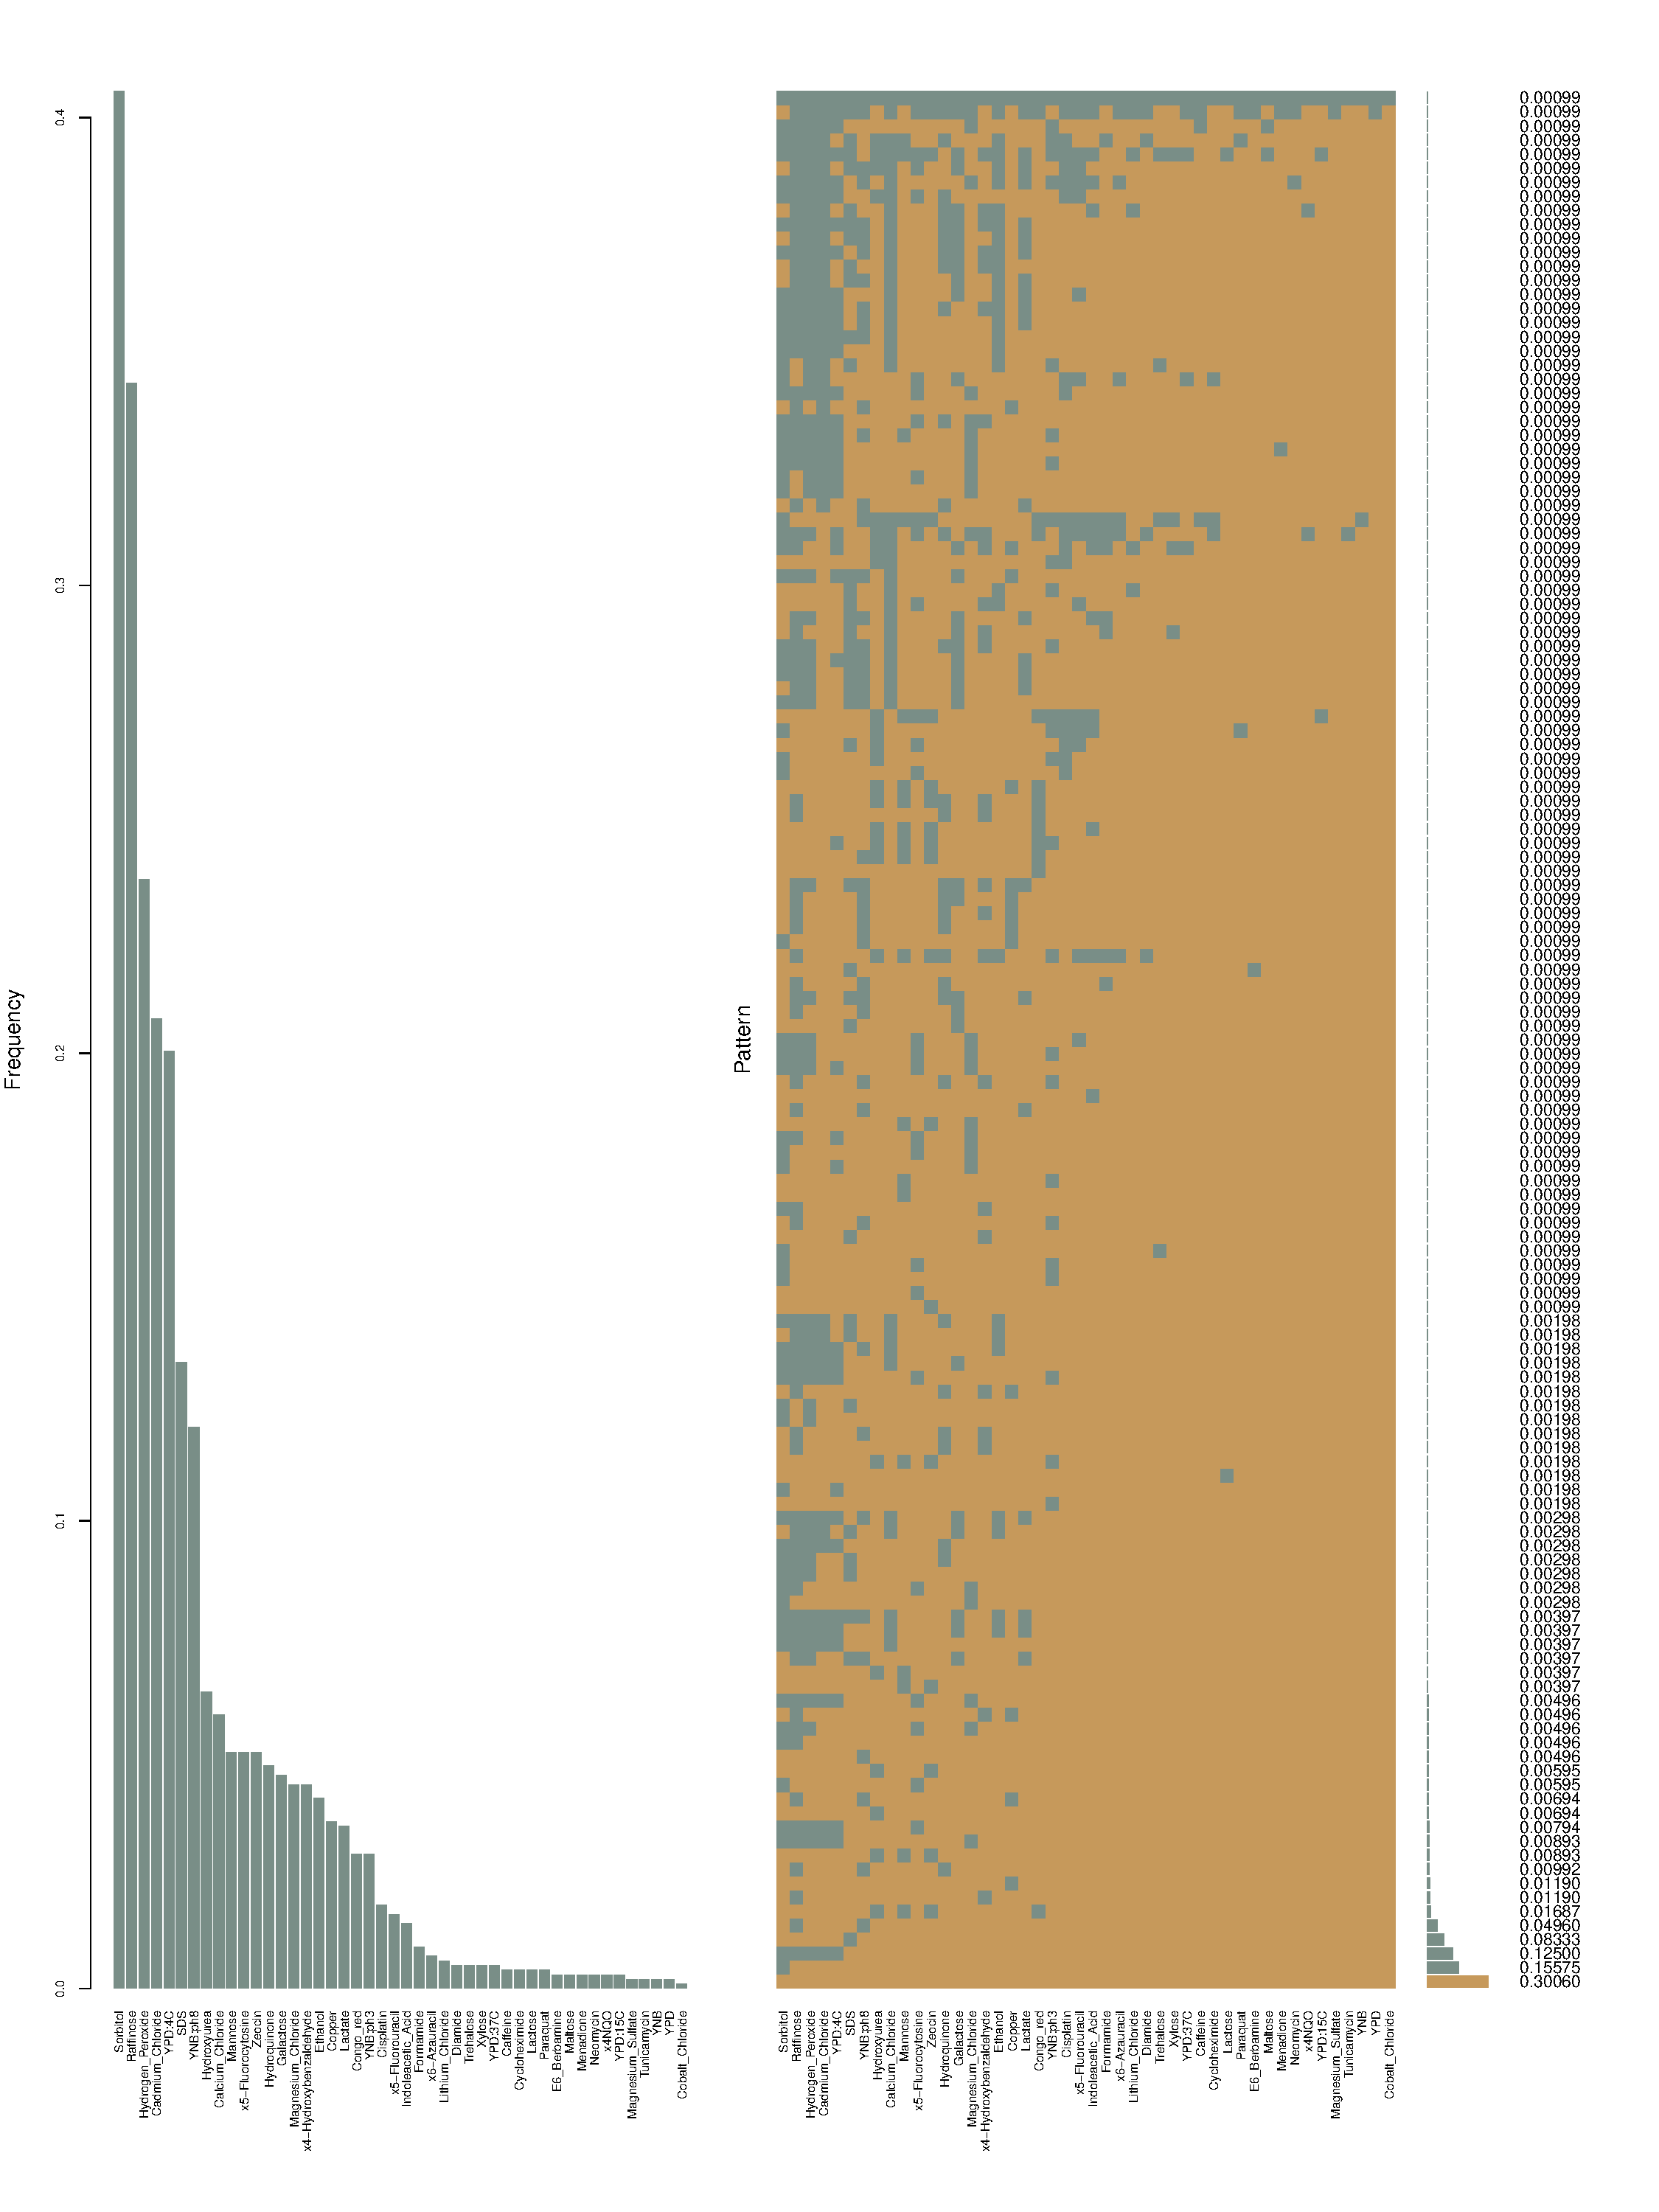
\includegraphics[trim = 0mm 0mm 0mm 0mm, clip, scale=0.8]{Chapter2/Figures/missing_data_pattern.pdf}
	\caption{\textbf{Full dataset}}
 		\label{fig:missingness-all}
	\end{subfigure}
	\\
	\begin{subfigure}[b]{1\textwidth}
		%\hspace{3cm}
		\center
	\includegraphics[trim = 0mm 0mm 0mm 20mm, clip, scale=0.8]{Chapter2/Figures/missing_data_pattern_simulated.pdf}\\
	\caption{\textbf{Simulated  dataset}}
 		\label{fig:missingness-sample}
	\end{subfigure}
	\caption[Frequencies and distributions of missing values in the yeast phenotype data]{\textbf{Frequencies and distributions of missing values in the yeast phenotype data.} In both panels, the aggregation plot (middle) depicts all existing combinations of missing (blue) and non-missing (orange) values in the traits. The bar chart on its right shows the frequencies of occurrence of the different combinations. The histogram on the top shows the frequency of missing values for each trait. (R Package: \emph{VIM} \citep{Templ2012}). (a) The full dataset contains normalised colony sizes for growth in 46 different conditions of 1,008 genotyped yeast segregants. 306 segregants are fully genotyped (bar chart, orange bar). (b) Fully-phenotyped dataset of 306 segreagants with simulated missing values based on the observed missingness pattern for the entire pool of 1,008 segregants.}
 	\label{fig:missingness}
\end{figure}

Determining if data is MAR or MNAR cannot be tested for formally and relies on approximate measures and assumptions based on the experimental procedures \citep{SchaferGraham2002,Garson2015,Templ2012}. Garson suggests to use significance tests of missingness \citeyear{Garson2015}. If it can be demonstrated that one or more variables in the dataset are significantly correlated with missing values, missingness may be predictable, which is the requirement for imputing MAR data. In order to test for predictable missingness, I created an indicator matrix for the phenotype matrix, where observed values where encoded as 0 and missing values as 1. For each of the 46 traits in the dataset I correlated the observed values across all samples with each column of the indicator matrix, i.e. the missingness patterns per trait. If all values were observed for a given trait i.e. all values in the incator matrix in this column were equal to 0, then the correlation between the trait and the missingness was set to NA. Figure~\ref{fig:missingnesscorrelations} shows these correlation patterns between the phenotypes and the missing values per trait. The p-values of the correlations were adjusted for multiple testing via Benjamini and Hochbergs method \citep{Benjamini1995} and only significant correlations are depicted (\(FDR < 0.2\).  For traits like cobalt chloride and magnesium sulfate where little data is missing, many entries are NA. Overall, fo a number of traits and missingness patterns, I found sufficient evidence for predictable missingness and MAR assumptions for further analyses were considered valid. Most importantly, for data with MAR, the missing data mechanism is ignorable for maximum likelihood based methods and no further adjustments for the mechansims have to be made in the modeling \citep{Rubin1976,Little1988}. Thus, the MAR assumption of missingness in the yeast data allows for imputation via the likelihood-based method of multiple imputation.


\begin{figure}[hbtp]
	\centering
	\includegraphics[trim = 0mm 0mm 0mm 0mm, clip, width=0.9\textwidth]{Chapter2/Figures/correlation_missingness.pdf}
	\caption[Correlations of observed phenotypes with missing data values]{\textbf{Correlations of observed phenotypes with missing data values}. For each trait, Spearman's rank correlation coefficient \(\rho\) was computed with each column of the indicator matrix of the phenotypes, containing 0 for observed values and 1 for missing values. The p-values of the correlations were adjusted for multiple testing according to Benjamini and Hochberg's method \citep{Benjamini1995}. The strength and the direction of significant correlations (\(FDR < 0.2\)) are depicted above., with the original phenotypes in rows and the indicator matrix of the phenotypes across columns. Unsignificant correlations are left blank. Grey squares indicate NA, i.e. columns in the indicator matrix for which no traits were missing when correlated with the observed values for a given trait.(R Package: \emph{corrplot}).}
 	\label{fig:missingnesscorrelations}
\end{figure}

\subsection{Imputation via MICE} 
Before imputing the missing values in the dataset, I wanted to understand which missing trait values can be reliable imputed and find the best parameter settings for the imputation. In order to do this, I needed a fully phenotyped dataset with the same structure as the yeast dataset, where missing values could be introduced, imputed and subsequently compared to the true values. I chose a simple approach and used the subset of 303 fully phenotyped samples and introduced missing values with a similar pattern of missingness as observed in the original dataset. The results for the real (Figure~\ref{fig:missingness-all}) and simulated (Figure~\ref{fig:missingness-sample}) dataset are similar in terms of frequencies and combination of missing/non-missing traits .

I used this simulated dataset as input to the imputation framework based on multiple imputation by chain equations (MICE) \citep{vanBuuren2011}. 
\paragraph{MICE.} MICE belongs to the general class of multiple imputation frameworks, where several imputed versions of the dataset are generated. The imputations are done separately for each variable. The imputed values are chosen from plausible values drawn from a distribution that is specific for that variable, in this case for each trait. This distribution is derived from the dataset \(X \in R^{n,p}\) itself,  with \(X = (X_\text{miss}, X_\text{obs})\) (the missing and the observed parts of the data), the binary indicator matrix for missingness \(M \in R^{n,p}\) and a set of predictor variables \(Z\). The MICE algorithm is usually divided into four steps \citep{Rubin1978,vanBuuren1999,Pigott2001,}:
\begin{enumerate}
\item Specify the posterior predictive density \(p(X_\text{miss} | Z, M)\) given the non-response mechanism  \(p(M | X)\)  and the complete data model  \(p X)\).
\item Draw imputations from this density to produce \(m\) complete data sets. 
\item Perform \(m\) complete-data analyses on each completed data matrix. 
\item Pool the \(m\) analyses results into final point and variance estimates.
\end{enumerate}
Garson describes the possibilty of switching step 3 and 4 \citeyear{Garson2015}, where the multiple imputations are first pooled and the subsequent analyses run on the pooled estimates. Employing this approach allows me to  obtain reliable imputation estimates while having to estimate the variance components via LiMMBo only once. As described in the previous chapter, LiMMBo strongly reduces the computation time for the variance decomposition, but it is still the time-consuming factor in the analysis. 

\noindent The two main choices in applying MICE for imputation have to be made in step 1: the form of the imputation model and the choice of predictor variables. 

\paragraph{Imputation model.} From the different imputation models available (examples described in \citep{vanBuuren2011}, I found multivariate data predictive mean matching (PMM) a fast and sensible imputation model. PMM is a semi-parametric method which preserves non-linear relations in the data \citep{Little1988,vanBuuren2011}. In brief, PMM finds the mean and covariance of the multi-variate distribution \(X\) with missing values (often simply based on the complete cases). Subsequently, for each incomplete sample it predicts the missing values \(X_\text{miss}\) based on \(X_\text{obs}\)  and the provided predictor variables \(Z\). In addtion, values of the complete samples for the same set of \(X_\text{miss}\) are predicted. The predicted values of the incomplete sample are than matched to the predicted values of the complete samples and the closest match is chosen. The imputed values for the incomplete sample are set to those of the closest match\citep{Little1988}. 

\paragraph{Predictor variables.} As many predictor variables as possible should be included in the imputation to obtain the least amount of bias and maximal certainty about the predictions \citep{Collins2001}. In addition, Schafer showed that using this strategy makes MAR assumptions more plausible \citep{Schafer1997}. However, not all predictors will be relevant and the choice of predictors can be done on a per-variable level. In order to select suitable predictors for each trait, I first computed the pairwise Spearman correlation coefficient \(\rho\) for all traits across the 303 fully-phenotyped segregants. Some of the traits like cadmium chloride or neomycin show very little correlation to any of the other traits, while many of the traits based on growth on different carbohydrate resources form a large cluster of moderate to strong correlation (Figure~\ref{fig:traitcorrelations}). 
I tested several sets of predictor variables, either using all traits as predictors or chosing predictors based on the pairwise \(\rho\) of the traits. For each trait, I included predictors that showed a correlation higher than a predefined threshold (\(\rho =\left\{0.1, 0.2, 0.3\right\}\). In addition, I restricted the predictors to traits that had been measured in at least 20\% of the samples in the dataset. This excluded cadmium chloride  (0.21\% missing), hydrogen peroxide (0.24\%), raffinose (0.34\%), sorbitol (0.41\%) and YPD:4C (0.20\%) as predictor variables, but did not exclude them from being imputed.

\begin{figure}[hbtp]
	\centering
	\includegraphics[trim = 0mm 0mm 0mm 0mm, clip, width=0.9\textwidth]{Chapter2/Figures/correlation_pheno_noNA.pdf}
	\caption[Pairwise correlations of 46 growth traits in \emph{Saccharomyces cerevisiae}]{\textbf{Pair-wise correlations of 46 growth traits in \emph{Saccharomyces cerevisiae}.} For each trait pair, Spearman's rank correlation coefficient \(\rho\) and the p-values of the correlation were computed. The p-values were adjusted for multiple testing according to Benjamini and Hochberg's method \citep{Benjamini1995}. The strength and the direction of significant correlations (\(p < 0.05\)) are depicted above. Unsignificant correlations are left blank. The traits are clustered based on complete-linkage clustering of \((1-\rho)\) as distance measurement (R Package: \emph{corrplot}).}
 	\label{fig:traitcorrelations}
\end{figure}

Further parameters for MICE are the number of multiple iterations \(m\) (set to \(m=20\)) and the number of iterations \(maxit\) (set to \(maxit=30\)). For each predictor set-up, I initiated MICE with the same seed for the random number generator to ensure comparability. After imputation, I evaluated the goodness of the imputation  by computing the Spearman correlation of the imputed values (averaged across iterations \(m\)) to the experimentally observed ones (Figure~\ref{fig:mice}). Traits where the imputed values correlated to the original ones by more then 95\% in at least one of the predictor set-ups were retained in the analysis. For five traits (cadmium chloride, hydrogen peroxide, raffinose, YNB:ph8, YPD:4C), no suitable predictors could be determined and these were excluded from further analyses (Figure~\ref{fig:mice}, red labels). For each trait, I chose the predictor scheme that yielded the highest correlation between the imputed and observed data for the imputation of missing values in the full dataset. Missing values were imputed in segregants that were phenotyped for at least 80\% of the traits. The final dataset contained 981 segregants with phenotypes for 41 traits each. 
 	
\begin{figure}[hbtp]
	\centering
	\includegraphics[trim = 0mm 0mm 0mm 0mm, clip, width=01\textwidth]{Chapter2/Figures/imputation_correlation_median_imputationvalue.pdf}
	\caption[Correlation between imputed and experimentally observed trait values]{\textbf{Correlation between imputed and experimentally observed trait values.} In the subset of 306 fully phenotyped samples, missing values were introduced and subsequently imputed via MICE. Different predictor sets were tested based on Spearman's rank correlation coefficient: traits were considered predictors if their correlation with the target trait was greater than a given threshold. For each predictor setup (all traits as predictors and predictors passing the corrleation threshold \(\rho =\left\{0.1, 0.2, 0.3\right\}\),   \(m=20\) multiple imputations and \(maxit=30\) iterations of MICE were conducted. The goodness of the imputation was evaluated by computing the correlation of the imputed values (averaged across iterations \(m\)) to the experimentally observed ones. Traits with at least one correlation greater than the 0.95 (black vertical line) were retained in the dataset. For traits labeled in red, the imputation was considered to be unreliable and the traits were excluded from further analyses (R Package: \emph{mice} \citep{vanBuuren2011}).}
 	\label{fig:mice}
\end{figure}



\newpage
\section{Multi-trait GWAS}
In order to show the utility of LiMMBo for joint high-dimensional phenotype analyses and demonstrate the advantages over single trait approaches, I analysed the imputed dataset both with single-trait and multi-trait GWAS.  

\subsection{LiMMBo increases power in detecting genetic associations}
For both analyses, I used a LMM where the sample-by-sample component of the random genetic effect is based on the genetic relationship matrix. To obtain an estimate of the genetic relationship matrix, I first pruned the genome-wide SNPs (11,623) for SNPs that are in LD with \(r^2 > 0.2\) within a window of 3kb. As the dataset is based on an F2 cross, LD structure estimation is not straight-forward and this window size is a simple estimate derived from a study on the population genomics of domestic and wild yeasts \citep{Liti2009}. The LD pruning reduced the SNP set for GRM estimation to 4,105 SNPs. The GRM was estimated via plink \cite{Chang2015}, which follows the method introcuded by Yang and colleagues \citep{Yang2011}. 

The first step in the mtGWAS is the trait-by-trait covariance estimation via LiMMBo. After xx bootstraps of ten traits each, every trait-trait combination was sampled and its covariance estimated at least three times. Together with the subsequent combination of the bootstrapped covariance estimates, the runtime was xxx. The combined trait-trait covariance estimates \tmat{C_g} and \tmat{C_n} were then used as input estimates for the second step in the mtGWAS, the mvLMM  (Eq.~\ref{eq:mvLMM}) across all genome-wide SNPs.  I used a mvLMM with a trait-design matrix corresponding to the any effect test, i.e. testing for an effect of the SNP on any of the traits compared to the null hypothesis of no association (\red{Section~\ref{sec:mvtests}}).

For the stGWAS, the trait-by-trait components of the random effects will be point estimates (\(\sigma_g\) and \(sigma_n\)) derived within the LMM and do not require \textit{a priori} estimation. The stGWAS is based on a univariate LMM (Eq.~\ref{eq:uvLMM}) per SNP, where each trait is mapped individually. To account for the number of univariate tests, the pvalues obtained from the stGWAS were adjusted for multiple testing by the effective number of conducted tests \(M_{eff}\). \(M_{eff}\) was introduced by Galwey and colleagues \citeyear{Galwey2009} and adjusts for multiple testing in a manner similar to the Bonferroni method \citep{Dunn1961}. However, it is less conservative, as it does not adjust for total number of tests, but the estimated, effective number of tests, taking correlation between the 
variables and tests into account:
\begin{equation}
 M_{eff} = \frac{(\sum^M_{i=1} \sqrt{\lambda_i})^2}{\sum^M_{i=1}\lambda_i},
\end{equation}
 where \(\lambda\) are the eigenvalues of the phenotypes' correlation matrix. To adjust for multiple testing in the stGWAS, the pvalues are multiplied with \(M_{eff}\) and set to 1 if the multiplication leads to values greater than one. \(M_{eff}\) for the 41 growth traits was estimated to be 33. 
 
In order to assess the significance of the single-trait and multi-trait analyses, I followed approaches of previous association studies in yeast crosses \citep{Brem2002,Brem2005,Ehrenreich2010}, where permuations are used to estimate empirical significance levels. With a conservative, theoretical singificance threshold of \(p_\text{t}10^{-5}\) at most one SNP is expected to be false positive with a total of \(s = 11,623\) SNPs . To find the empircal FDR corresponding to this threshold, I generated \(p = 50\) permutations of the genotypes and fitted the LMM against these permutations. The pvalues obtained from these analyses were then combined and sorted in increasing order. The pvalue observed at position \(p_\text{t} \times s \times p\) is used as the empirical FDR. For the mtGWAS this threshold is at \(\text{FDR}_{\text{mtGWAS}} =1.2e-05\)  lower than for the stGWAS \(\text{FDR}_{\text{stGWAS}} =8.6e-06\).

Fig.~\ref{fig:GWAS-yeast} shows the manhattan plot of the multi-trait and single-trait GWAS. On several chromsomomes, mtGWAS peaks (blue) are observed whereas no stGWAS peaks (orange; minimum p-value per SNP across all 41 stGWAS, adjusted for multiple testing) can be detected. This results demonstrates the increase in power on real data when jointly modeling the traits, confirming the results obtained from the theoretical power analysis (Section~\ref{sec:power}). 

\begin{figure}[hbtp]
	\centering
	\includegraphics[trim = 0mm 0mm 0mm 0mm, clip, width=0.9\textwidth]{Chapter2/Figures/manhattan.png}
	\caption{\textbf{Manhattan plot of pvalues from stGWAS and mtGWAS.} The stGWAS pvalues were adjusted for multiple testing by the effective number of tests (\(M_{eff} = 33\) and only the minimum adjusted p-values across all 41 traits per SNP are shown. The significance line is drawn at the empirical \(\text{FDR}_{\text{stGWAS}} =8.6e-06\).}
 	\label{fig:GWAS-yeast}
\end{figure}

To quantify the increase in power, I counted the number of loci detected above the permutation-based significant thresholds for both the stGWAS and the mtGWAS. However for a fair comparison of the two methods, I also needed to account for linked loci, with the long LD structure present in the F2 cross potentially merging nearby signals. As for the estimation of the GRM, I used \textit{plink} for LD pruning of the SNPs, chosing a strict threshold of \(r^2 > 0.2\) and increasing LD window sizes ranging from 3 to 100kb.  The maximal LD window of 100kb covers between 6\% (chromosome 4) and 43\% (chromosome 1) of total chromosome length (yeast genome assembly: ScerevisaeR64-1-1 \red{\citep{}}). Table \ref{tab:sigsnps} shows that the increase in power is present from narrow to broad LD pruning, with on average 29\% more significant loci in mtGWAS.

% Table generated by Excel2LaTeX from sheet 'LDGwasYeast'
\begin{table}[htbp]
  \centering
  \caption{\textbf{Comparison of significant loci in stGWAS and mtGWAS.} In column `All SNPs', the absolute number of SNPs beyond the significance threshold for multitait and singletrait GWAS as well as their ratio (multitrait:singletrait) are depicted. In order to limit the potential bias in the counting of the loci, introduced by different degrees of linkage disequilibrium (LD) for different loci, the genome-wide SNPs were LD pruned and the ratio of significant SNPs determined for five different LD window sizes. The maximal LD window covering between 6\% (chromosome 4) and 43\% (chromosome 1) of total chromosome length.}
    \begin{tabular}{lrrrrrr}
    \toprule
          & \multicolumn{1}{c}{All SNPs} & \multicolumn{5}{c}{LD pruned with $r^2 > 0.2$ } \\
\cmidrule{3-7}          &       & 3kb   & 10kb  & 30kb  & 50kb  & 100kb \\
    \midrule
    NrSNPs & 11623 & 4105  & 1028  & 264   & 161   & 107 \\
    multitrait & 1132  & 384   & 101   & 24    & 15    & 9 \\
    singletrait & 695   & 275   & 72    & 20    & 13    & 7 \\
    multitrait:singletrait & 1.63  & 1.4   & 1.4   & 1.2   & 1.15  & 1.29 \\
    \bottomrule
    \end{tabular}%
  \label{tab:sigsnps}%
\end{table}%

\subsection{}
As well as providing an increase in power, the mtGWAS inherently provides effect size estimates across all phenotypes for a particular locus, allowing a richer exploration of the underlying biology. 
To analyse the relationship between traits and SNPs based on their effect size estimates, I filtered the genome-wide SNPs for SNPs that fell within a gene body (yeast genome assembly: ScerevisaeR64-1-1).  I pruned these 8,135 SNPs for SNPs in LD  with \(r^2 > 0.2\) and within a 3kb window (1,412 SNPs). Lastly, I filtered for SNPs passing the \(\text{FDR}_\text{mtGWAS} =1.2e-05\) yielding 210 SNPs across 15 out of the 16 yeast chromosomes. Chromsome V is the only chromosome without significantly associated SNPs for the mtGWAS (Figure~\ref{fig:GWAS-yeast}). 

To find groups of SNPs and traits with similar effect size estimates, I clustered the effect size estimates of these SNPs both across traits and SNPs. I used the hierarchical clustering algorithm \textit{pvclust} that provides bootstrap-based p-values as a measure for the stability of a given cluster \cite{Suzuki2006}. The clustering was based on the Pearson correlation coefficients, with 50,000 bootstraps for traits and 10,000 for SNPs. Clusters with \(p < 0.05\) were considered significant. A heatmap effect size estimates and the clustering results is depicted in Figure~\ref{fig:effectsizes}. Ignoring the clustering for a first impression of the results, one can clearly see that most SNPs have significant non-zero effects in more than one trait. Furthermore some traits have contributions from across the genome, many of which are xenobiotic growth conditions e.g. zeocin \cite{Krol2015} and neomycin \cite{Alamgir2010}. Turning the attention to the clustering,  Figure~\ref{fig:effectsizes} shows that the clusters are driven by specific combinations of loci and traits, and would be hard to achieve from a single trait analysis. 

There are a number of significant clusters for traits (Figure~\ref{fig:effectsizes}, coloured row dendrogram), including classically linked carbon metabolism sources (lactose, lactate and ethanol), and other clusters which there is literature support for. For example, I found a study showing gene expression changes for genes involved in DNA replication upon treatment with hydroxyurea and 4-nitroquinoline-l-oxide (x4NQO) \cite{Elledge1990}, two substances that form stable cluster. Supporting the cluster of trehalose and sorbitol is a previous results, which demonstrated these sugars to have synergistic effects on viability in yeast \cite{Hua2015}. For other clusters, such as SDS and Hydroxybenzaldehyde or magnesium sulfate and berbamine I was unable to find literature support but this could be a candidate clustering of these growth phenotypes for further investigation. 

For the clustering across SNPs, I discovered 31 stable clusters (Figure~\ref{fig:effectsizes}, coloured column dendrogram), many of which represent linked loci. However, there are nine clusters (Figure~\ref{fig:effectsizes}B, grey boxes) spanning multiple chromosomes, and many clusters with disjoint regions across a chromosome. Some SNP clusters have suggestive common annotation, such as c\textit{cluster a} which has two members of the nuclear pore complex, and \textit{cluster b} which has a common set of vesicle associated genes (Fig.~\ref{fig:GWAS-yeast}B, labeled boxes). The small size of clusters inhibited any systematic gene ontology based enrichment, but the ability to explore both multiple traits and multiple loci from the mtGWAS provides stimulating hypothesis generation. 

\begin{figure}[hbtp]
	\centering
	\includegraphics[trim = 0mm 150mm 0mm 0mm, clip, width=0.9\textwidth]{Chapter2/Figures/effectsizes.png}
	\caption{\textbf{mtGWAS effects size estimates.} Effect size estimates of LD-pruned (3kb window, \(r^2 > 0.2\)), significant SNPs located within a gene were clustered by loci and traits (both hierarchical, average-linkage clustering of Pearson correlation coefficients ). Stable clusters (pvclust \( p < 0.05\)) are marked in orange. Grey boxes indicate stable SNP clusters spread across at least two chromosomes. a and b label two clusters for which suggestive common annotation was found, for details see test.}
 	\label{fig:GWAS-yeast}
\end{figure}


%\section{LiMMBo for multi-trait GWAS and beyond}
\label{section:conclusion-limmbo}
In this chapter, I introduced \gls{limmbo}, a new method for the multivariate analysis of large trait numbers, which uses a bootstrap method to estimate complex trait covariance matrices. The main benefit of \gls{limmbo} is that it scales to \num{100}s of phenotypes, both because of its inherent sub-sampling method and that the most computationally intense part of the method can be parallelised. To take advantage of the parallelisation, I implemented an optional automatic detection for multiple cores which allows for easy realisation of this process via the \textit{Parallel Python Software} \citep{PPSoftware}. In practice, this means that trait sizes up to 30 or 40 can be in hours, rather than taking several days as for standard \gls{reml}-based methods. Most notably, complex datasets of \num{100}s of traits, which is out of scope for the \gls{reml} approaches, are feasible when using \gls{limmbo}. I showed that the covariance matrices estimated via \gls{limmbo} are as good an estimator of the real covariance matrices as the ones of the validated \gls{reml} approach. Consequently, these covariance matrices produce well calibrated null models when used in \gls{lmm} for \gls{gwas}, showing the validity of the approach. To show the advance of \gls{limmbo}, I demonstrated the power gain for multi-trait \gls{gwas} of high-dimensional phenotypes with \gls{limmbo} over standard single-trait models across a wide range of phenotype architectures. I made \gls{limmbo} accessible as an open source, python module at \url{https://github.com/HannahVMeyer/LiMMBo/tree/master/limmbo}. \gls{limmbo} is compatible with the LIMIX package for linear mixed models \citep{Lippert2014}.  

The bootstrapping has proven powerful to reduce the computational complexity for estimating the covariance parameters and made the analysis of complex datasets with high trait numbers possible. However, so far, I only examined the complexity and calibration dependent on the size of the overall phenotype set \(P\). Of additional interest would be understanding the (co-)dependence of the bootstrap size \(s\),  the number of bootstraps \(b\) and the  co-sampling of traits \(c\). Based on already simulated datasets, a systematic comparison of the run times, covariance estimates and calibration of different combinations of \(s\) and \(b\) could be conducted. For each of these combinations, different thresholds for \(c\) could be examined.

Much of the attraction of linear mixed models in genetics has been their ability to model complex genetic relatedness. As described by \citep{Kang2010} and demonstrated in this chapter, simple linear models are not suitable for analysing phenotypes with complex underlying genetic relatedness, whereas linear mixed models with the covariance matrices estimated by \gls{limmbo} are appropriate and possible up to \num{100}s of traits. Complex relatedness in populations is wide-spread in plant and animal breeding \citep{Bolormaa2014,Yang2014}, and increasingly common in human bottleneck populations \citep{Tachmazidou2013}. Furthermore, as the population numbers increase in human genetics, complex cryptic relationship structures are more prevalent \citep{Reich2001}, meaning that methods such as \gls{limmbo} will be more applicable in the future in human genetics. 

Trait-by-trait covariance matrices are useful for a variety of high dimensional big data problems across genomics, from statistical genetics to single cell analysis. The ability to accurately estimate large trait-by-trait covariance matrices using this bootstrap method may be applicable to more domains than \gls{gwas}, e.g. many gene expression studies use covariance matrices. Previous work from \citet{Schaefer2005} showed the large gene dimensions coupled with small(er) sample sets means that empirical covariance matrices could not be accurately estimated; other investigators \citep{Ledoit2004,Furrer2007,Bickel2008} used shrinkage methods to create valid covariance matrices. The work from \citet{Teng2009} uses subsampling but with strong shrinkage priors to generate the final covariance matrix. By fitting the average to closest true covariance, \gls{limmbo} ensures positive-semidefiniteness of the covariance while avoiding ill-conditioned matrices, which usually introduces large biases in the final use of these models. Thus, covariance estimation based on the method implemented in \gls{limmbo} might be applicable and useful in other areas of quantitative genetics.  

The ability to generate large cohorts of well phenotyped and genotyped individuals has forced the development of many new methods in statistical genetics. With the advent of genotyped human cohorts up to \num{500000} individuals with over \num{2000} different traits \citep{Sudlow2015}, and plant phenotyping routinely in the \num{1000}s of individuals from structured crosses with \num{100}s of (image-based) phenotypes \citep{Atwell2010,Yang2014}, new informative and scaleable methods are needed. \gls{limmbo} extends the reach of linear mixed models into this new regime, allowing for new complex genetic associations to be made.



\bibliography{myLibrary2}
\bibliographystyle{ebi}

\beginsupplement
\section{Quality control: genotyping}

\begin{figure}[hbtp]
	\centering
	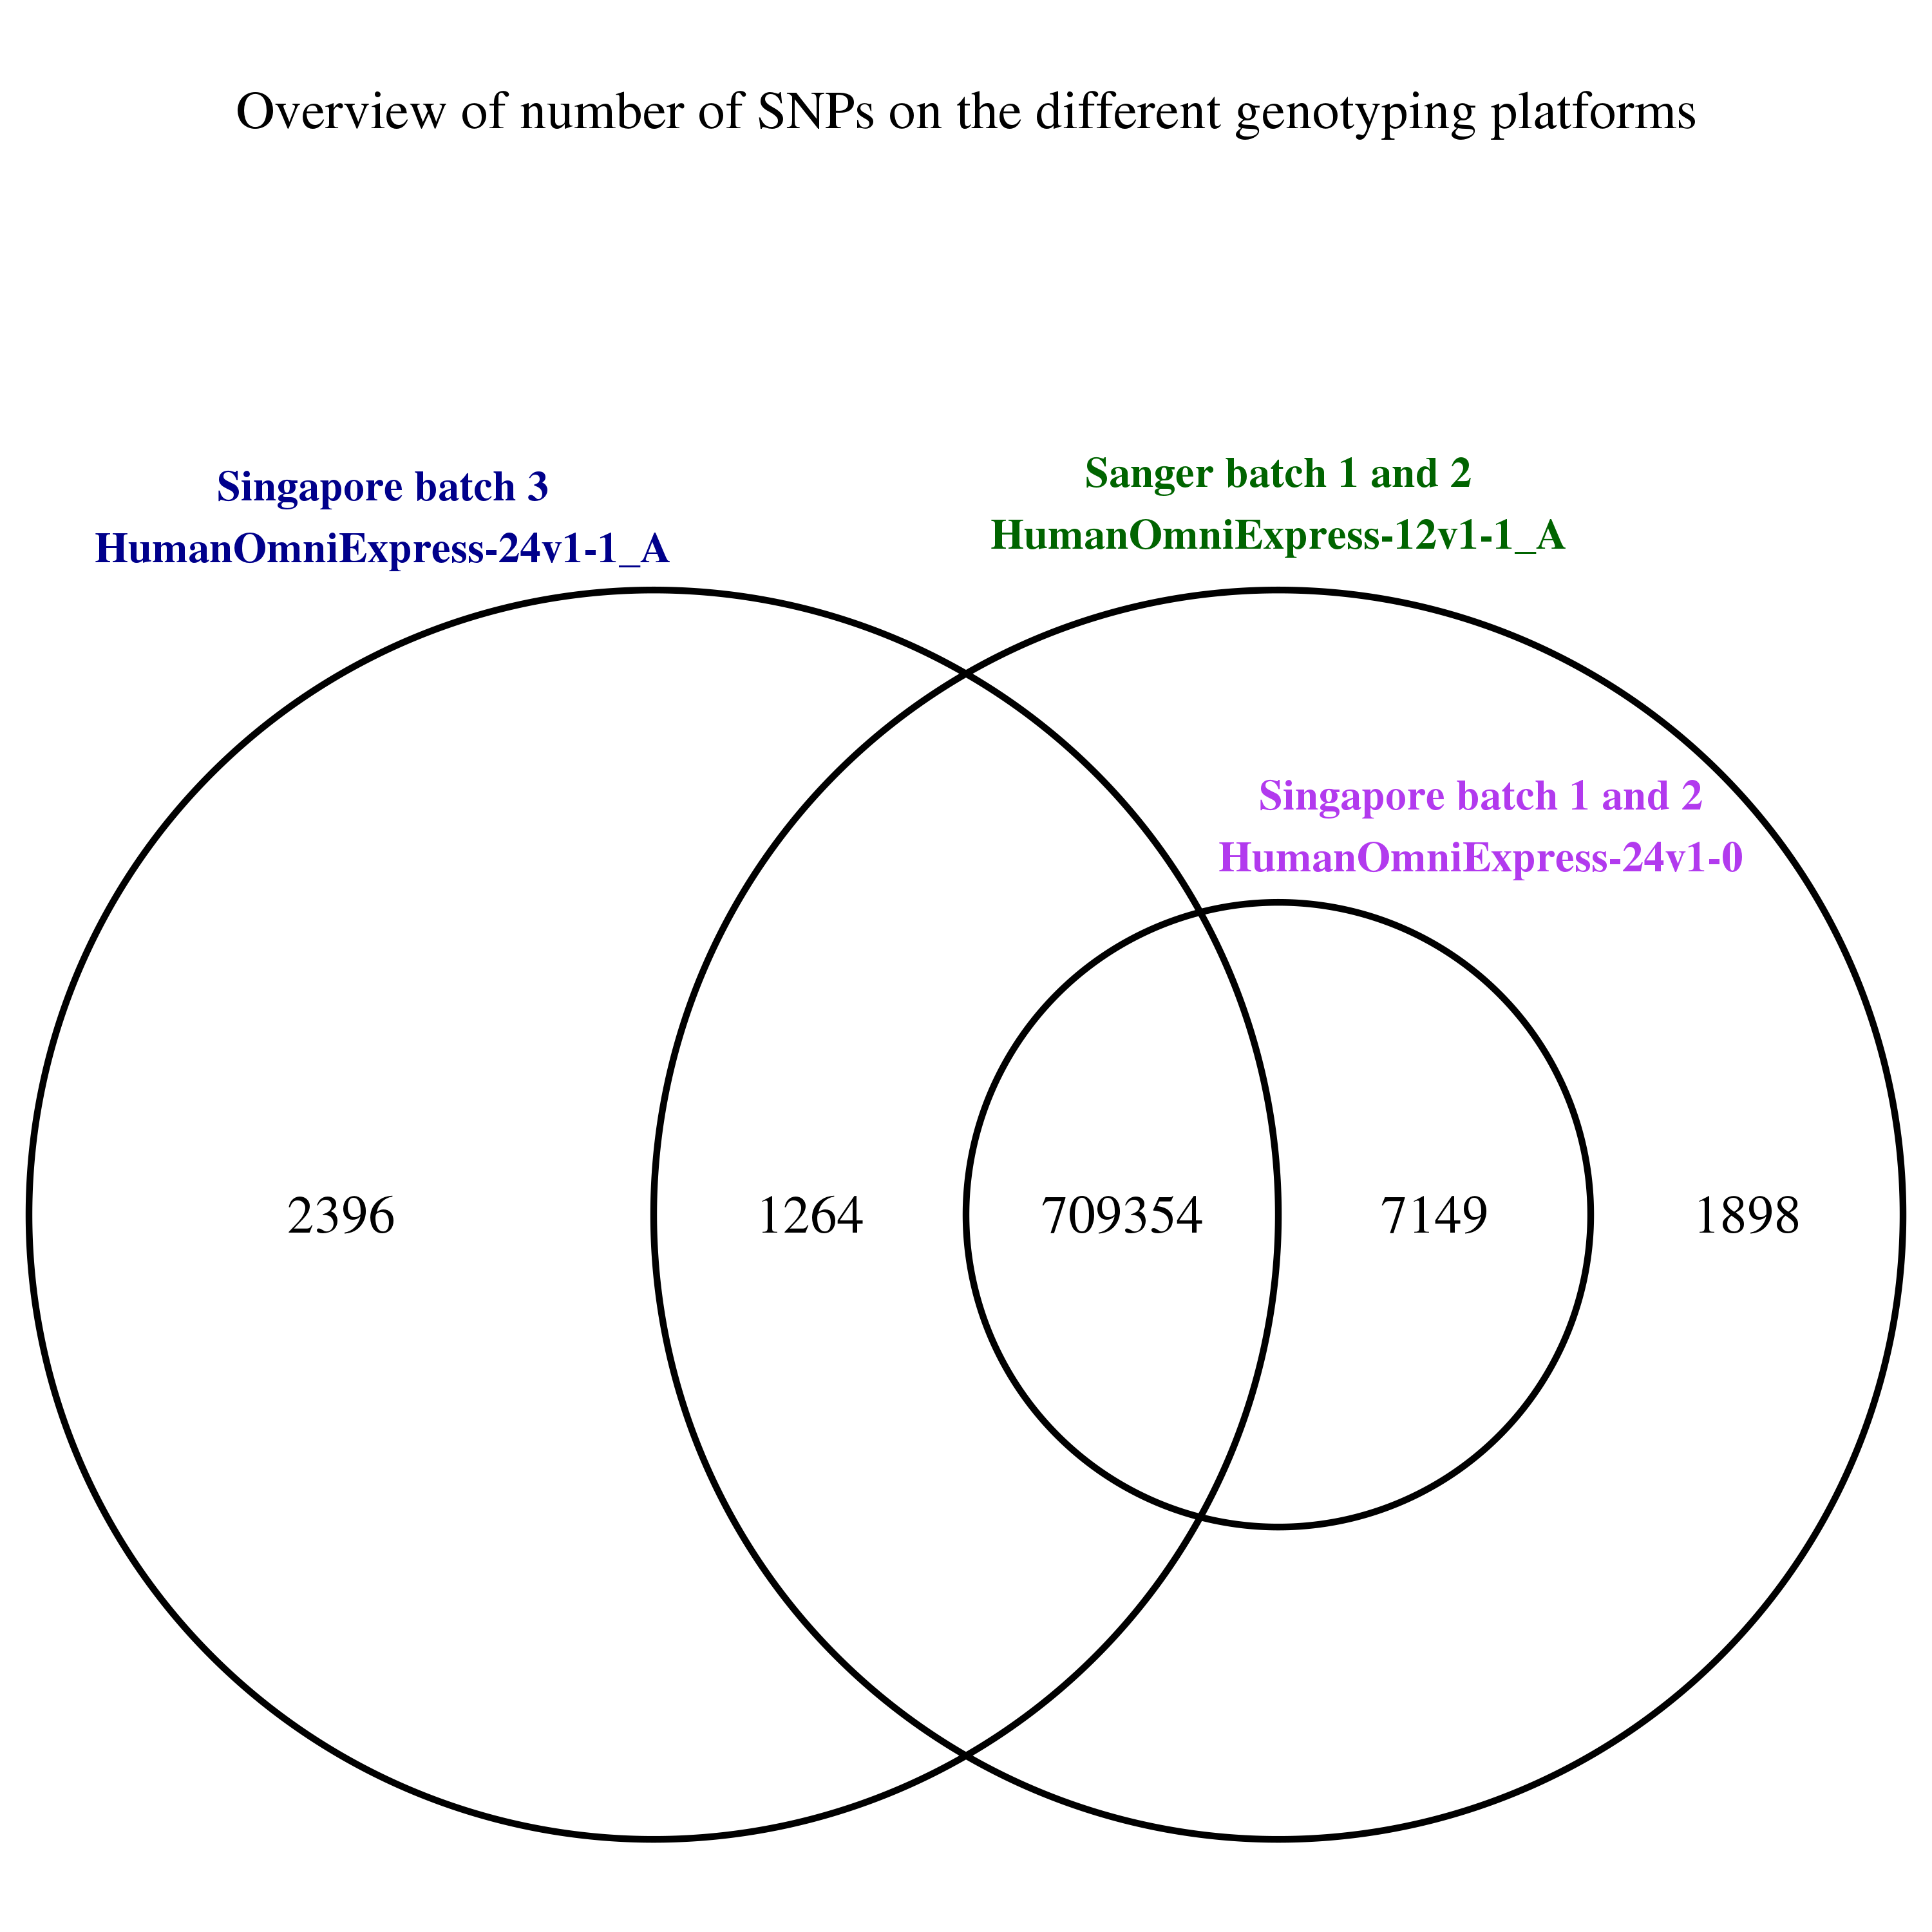
\includegraphics[trim = 0mm 0mm 0mm 20mm, clip, width=0.8\textwidth]{Figures/Venn_genotyping_batches.png}
	\caption{\textbf{.} .}
 	\label{fig:probeoverlap}
\end{figure}

\begin{figure}[hbtp]
	\centering
	\includegraphics[trim = 0mm 0mm 0mm 20mm, clip, width=0.8\textwidth]{Figures/SampleQC.pdf}
	\caption{\textbf{.} .}
 	\label{fig:sampleQC}
\end{figure}

\begin{figure}[hbtp]
	\centering
	\includegraphics[trim = 0mm 0mm 0mm 20mm, clip, width=0.8\textwidth]{Figures/SNPQC.pdf}
	\caption{\textbf{.} .}
 	\label{fig:SNPQC}
\end{figure}

\begin{figure}[hbtp]
	\centering
	\includegraphics[trim = 0mm 0mm 0mm 20mm, clip, width=0.8\textwidth]{Figures/kinshipQC.pdf}
	\caption{\textbf{.} .}
 	\label{fig:kinshipQC}
\end{figure}

\section{Quality control: imputation}

\begin{figure}[hbtp]
	\centering
	\includegraphics[trim = 0mm 0mm 0mm 20mm, clip, width=0.8\textwidth]{Figures/perBatchSNPsperChr.pdf}
	\caption{\textbf{.} .}
 	\label{fig:imputeQC}
\end{figure}
\end{document}


